\cotefile{64}
\scanpage{2}
\mspage{I}
% pencil annotation at upper left: (40)
% archive foliation: 1 (lower left)
\unsure{Fourbis} combinatoires

(ens. à 4 éléments, carrés, octaèdres,
modules libres de rang 2 sur $\mathbb{Z}/4\mathbb{Z}$).

\scanpage{3}
\mspage{\unsure{1}}
% archive foliation: 2
1. Ens. à quatre éléments.

Un ens. à quatre éléments $I$ est muni canoniquement d'une structure
\deleted{\unsure{d'espace vectoriel de}}\inserted{d'espace affine de}
\deleted{\unsure{de}} dim 2 sur $\mathbb{F}_2$, i.e. d'un sous-groupe
$V\subset \unsure{\mathcal{G}_I|\mathfrak{S}_I}$, isomorphe (non can.!) à $\mathbb{F}_2^2$,
tel que l'action de $V$ sur \deleted{\unsure{$\mathbb{F}$}} $I$ en fasse un torseur.
Le sous-groupe $V\subset \unsure{\mathcal{G}_I|\mathfrak{S}_I}$ est le seul sous-groupe
distingué abélien $\ne\{0\}$, \deleted{\unsure{c'est aussi}} il est son propre
\deleted{normalisateur}\inserted{centralisateur}, i.e.
$\unsure{\mathcal{G}_I|\mathfrak{S}_I}/V$ opère fidèlement sur $V$, en fait on a
\[
 \unsure{\mathcal{G}_I|\mathfrak{S}_I}/V
 \xrightarrow{\sim}\operatorname{Aut}_{\mathrm{gr}}(V)
 =\operatorname{Aut}_{\mathbb{F}_2\text{-vect}}(V)
 \xrightarrow{\sim}\deleted{\unsure{\operatorname{Aut}}}\unsure{\mathcal{G}_J|\mathfrak{S}_J}
\]
où $J=V^*$, la suite ex.te
\diagram{\begin{tikzcd}
1 \arrow[r] & V \arrow[r,dash] & \unsure{\mathcal{G}_I|\mathfrak{S}_I} \arrow[r] & \unsure{\mathcal{G}_J|\mathfrak{S}_J} \arrow[r] & 1
\end{tikzcd}}
étant \deleted{\unsure{isomorphe}}\inserted{identique} à la suite
\diagram{\begin{tikzcd}
1 \arrow[r,dash] & \underset{\text{translations}}{V} \arrow[r] &
\operatorname{Aut}_{\mathrm{aff}}(I) \arrow[r] & \operatorname{Aut}_{\mathbb{F}_2}(V) \arrow[r,dash] & 1 .
\end{tikzcd}}

Les \inserted{trois} éléments de $J=V^*$ correspondent aux trois
partitions de type $(2,2)$ de $I$ \inserted{ou aux trois involutions sans pt fixe}
(on peut l'interpréter \inserted{ainsi} car les éléments de $J$ correspondent
aux droites \inserted{vectorielles} de $V^*$, qui définissent
\deleted{\unsure{les}} donc des \deleted{\unsure{3}} relations d'équivalence
dans $I$, vers des espaces affines quotients de dim 1) --- les classes
intervenant dans l'ensemble de ces \inserted{3} relations d'équivalence
correspondent aux 6 \deleted{\unsure{paires}}\inserted{\unsure{parties}}
à deux éléments de $I$, ou encore aux 6 droites affines dans l'espace affine $I$,
l'application
\diagram{\begin{tikzcd}
\mathcal{P}_2(I) \arrow[r] & \mathcal{P}_{2,2}(I) \\
A \arrow[r,mapsto] & \{A,I\setminus A\}
\end{tikzcd}}

\scanpage{4}
% archive foliation: 3
s'identifiant à l'application qui associe à la droite affine dans $I$ sa
\uline{direction}, qui est une droite de l'espace des translations $V$.
La fibre d'un $\unsure{j}\in\mathcal{P}_{2,2}(I)$, i.e. \unsure{l'ens.} des
\deleted{\unsure{ses}} deux classes \inserted{de cette partition}, est donc
l'espace quotient $I/(D_j=\{0,j\})$.

Le foncteur ``oubli de la structure'' qui va de la catégorie des espaces affines
de dim 2 sur $\mathbb{F}_2$, vers la cat. des ensembles à quatre éléments
\margin{\unsure{on ne prend pour morphismes} les flèches \uline{inversibles}}
\diagram{\begin{tikzcd}
\operatorname{Aff}_2(\mathbb{F}_2) \arrow[r,"\approx"] & (\operatorname{Ens}_4)
\end{tikzcd}}
est une équivalence des catégories.
\inserted{et $=$ un iso, si on définit la notion d'espace affine sur $\mathbb{F}_2$
par la donnée d'une structure sur un $I$ tout seul
(donnée d'un sous-groupe de $\unsure{\mathcal{G}_I|\mathfrak{S}_I}$ \unsure{gr de tr.})}

Je dis que le foncteur
\diagram{\begin{tikzcd}
(\operatorname{Ens}_4) \arrow[r] & (\operatorname{Gr}) \\
I \arrow[r,mapsto] & \unsure{\mathcal{G}_I|\mathfrak{S}_I}
\end{tikzcd}}
est pleinement fidèle, ou encore que pour $\forall I$,
$\unsure{\mathcal{G}_I|\mathfrak{S}_I}$ a un centre trivial et tout automorphisme de
$\unsure{\mathcal{G}_I|\mathfrak{S}_I}$ est intérieur.
\deleted{\unsure{Pour}}\inserted{\unsure{Il}}
\unsure{suffirait} bien sûr de l'énoncer pour $\unsure{\mathcal{G}_4|\mathfrak{S}_4}$ !).

On va définir pour ceci un foncteur quasi-inverse
\diagram{\begin{tikzcd}
\deleted{\unsure{(\operatorname{Ens})}}(\operatorname{Gr})'
\arrow[r] & (\operatorname{Ens}_4)
\end{tikzcd}}
sur l'image essentielle $(\operatorname{Gr})'$ des groupes isomorphes à
$\unsure{\mathcal{G}_4|\mathfrak{S}_4}$.
Si on a un tel groupe $G$, on considère l'ens
\deleted{\unsure{des}}\deleted{\unsure{sous-groupes de}}
\inserted{3-sous-gr.} de Sylow, il y en a exactement quatre !
Pour \unsure{préciser} ce point et réciproquement

\scanpage{5}
\mspage{2}
% archive foliation: 4
la structure de torseur sur cet ens, on considère le sous-groupe abélien distingué
\deleted{\unsure{le}} non nul $V$ de $G$, de sorte que $V$ est un vectoriel
de rang 2 sur $\mathbb{F}_2$ et $G/V\xrightarrow{\sim}\operatorname{Aut}_{\mathbb{F}_2}(V)$,
et on note que les \inserted{3-}sous-groupes de Sylow de $G$ correspondent aux
``relèvements'' de l'unique 3-sous-groupe de Sylow de
$G/V\simeq\unsure{\mathcal{G}_J|\mathfrak{S}_J}$.
($J=V^*$), savoir
$\unsure{\mathcal{G}_J|\mathfrak{S}_J}^+=[\unsure{\mathcal{G}_J|\mathfrak{S}_J},\unsure{\mathcal{G}_J|\mathfrak{S}_J}]$,
d'indice 2 dans $\unsure{\mathcal{G}_J|\mathfrak{S}_J}$.
\deleted{\unsure{Comme}} L'ens. $I_G$ des 3-sous-groupes de Sylow de $G$
s'identifie donc à l'ens des scindages de l'extension
\diagram{\begin{tikzcd}
1 \arrow[r,dash] & V \arrow[r,dash] & G^+ \arrow[r] & \unsure{\mathcal{G}_J|\mathfrak{S}_J}^+ \arrow[r,dash] & 1
\end{tikzcd}}
du 3-groupe $\unsure{\mathcal{G}_J|\mathfrak{S}_J}^+$ par le 2-groupe $V$.
Sur l'ens. de ces scindages, $V$ opère donc transitivement par autom. intérieurs,
d'ailleurs
$V^{\unsure{\mathcal{G}_J|\mathfrak{S}_J}^+}=\{0\}$
($\unsure{\mathcal{G}_J|\mathfrak{S}_J}^+$ est le groupe des permutations circulaires sur
$V^*=J$), donc $I_G$ est bien un torseur sous $V$.

Quand on part de $I$ et \deleted{\unsure{$G$}} $G=\unsure{\mathcal{G}_I|\mathfrak{S}_I}$,
on trouve une bijection
\diagram{\begin{tikzcd}
I \arrow[r,dash] & I_G \\
i \arrow[r,mapsto] & \unsure{\mathcal{G}_{I\setminus\{i\}}|\mathfrak{S}_{I\setminus\{i\}}}^+
\end{tikzcd}}
$=$ unique 3 ss-gr. de Sylow de $\unsure{\mathcal{G}_I|\mathfrak{S}_I}$ qui fixe $i$.

Ainsi \deleted{\unsure{les applications}} foncteurs
$I\mathbin{-}\unsure{\mathcal{G}_I|\mathfrak{S}_I}$,
$G\mathbin{-}I_G$, et le composé $I\longrightarrow I(\unsure{\mathcal{G}_I|\mathfrak{S}_I})$,
on a un iso avec le \deleted{identité} foncteur identique,

\scanpage{6}
% archive foliation: 5
Pour le composé dans l'autre sens, on trouve que $G$ opère sur l'ens $I_G$
de ses \unsure{trois} ss-groupes de Sylow par autom. intérieurs, d'où
\[
 G\xrightarrow{\sim}\unsure{\mathcal{G}_{I_G}|\mathfrak{S}_{I_G}}
\]
qui est un iso.

Éléments de $\unsure{\mathcal{G}_I|\mathfrak{S}_I}$.

a) 1

b) Les \inserted{trois} éléments \deleted{non nuls de}\inserted{de} $V^*$,
qui forment une orbite $J$ sous $\unsure{\mathcal{G}_I|\mathfrak{S}_I}$, et correspondent
aux élém. de $\mathcal{P}_{2,2}(I)$.
\margin{``translations'' (non nulles) [Sym. p.r. aux trois axes du cube]}

c) Les \deleted{\unsure{trois|deux}} 8 éléments d'ordre 3, se répartissent en
\deleted{quatre}\inserted{deux} \deleted{torseurs} paquets de 4 qui sont des torseurs
(à gauche ou à droite au choix) sous $V$, suivant les deux éléments
$\ne1$ de $\unsure{\mathcal{G}_J|\mathfrak{S}_J}^+$.
L'ens de ces éléments s'identifie ainsi à
\[
 I\times\underline{\omega},\qquad
 \text{où }\underline{\omega}=\omega(J)\;(\simeq\omega(I))
\]
par l'application qui associe à tout
$\rho\in\unsure{\mathcal{G}_I|\mathfrak{S}_I}$ d'ordre 3 son unique pt fixe dans $I$
(ou encore, le sous-gr. de Sylow qu'il engendre), \uline{et} l'orientation
qu'il détermine \deleted{\unsure{ainsi}} ou encore son image dans
$\unsure{\mathcal{G}_J|\mathfrak{S}_J}^+$.
\margin{``rotations'' (ayant un pt fixe et un seul, lequel transforme $I$ en
vectoriel isom. à $V$) [``rotations-sommets'' du cube]}

d) Les \deleted{\unsure{8}}\inserted{6} éléments
\deleted{\unsure{de}}\inserted{d'ordre 2} de $\unsure{\mathcal{G}_I|\mathfrak{S}_I}$
qui s'envoient dans $\unsure{\mathcal{G}_J|\mathfrak{S}_J}^-$, en correspondance 1-1
avec l'ens $\mathcal{P}_2(I)$ --- ce sont les \uline{transpositions} dans $I$
qui se groupent en 3 \deleted{\unsure{paires}} paires, pour la transposition
$\tau_A$, $\tau_{A'}$ \deleted{\unsure{est}} $(A'=I\setminus A)$ est l'unique
\inserted{autre} élément d'ordre 2 tel que $\tau_A\tau_{A'}\in V^*$.
\margin{``réflexions'' (ayant du moins une \deleted{\unsure{paire}} droite de pts fixes)
[``rotations-arêtes'' du cube]}

e) Les 6 éléments d'ordre 4 de $\unsure{\mathcal{G}_I|\mathfrak{S}_I}$, correspondent aux
6 ordres circulaires sur $I$. Pour
\margin{[``rotations-faces'' du cube]}

\scanpage{7}
\mspage{3}
% archive foliation: 6
$\unsure{u}$ \deleted{\unsure{tel}} on a $u^2\in V^*$, donc on a une application
\[
 \operatorname{Circ}(I)\longrightarrow V^*
\]
de degré 2 (qui définit donc une structure de \uline{cube}, avec $V^*$ comme
ens des directions des faces, $\operatorname{Circ}(I)$ comme l'ens des six faces
--- en fait ce cube est canoniquement orienté ; cf plus bas.

\margin{\textcircled{$*$} On peut dire aussi que les six éléments d'ordre 4
se répartissent par paires $\{u,u^{-1}\}$ suivant les trois sous-groupes
\inserted{cycliques} d'ordre 4 \deleted{de} $G=\unsure{\mathcal{G}_I|\mathfrak{S}_I}$,
\unsure{biunivoquement} \deleted{\unsure{en}}\inserted{\unsure{en corresp.}}
avec les éléments de $V^*$ \inserted{(voir au-dessous !)}.}
\margin{$I$ est l'ens des quatre diagonales du cube,}

L'isom. canonique
\[
(\omega)\qquad \underline{\omega}(I)\simeq\underline{\omega}(J)
\]
On a
\[
 \unsure{\mathcal{G}_{I\,\mathrm{ab}}|\mathfrak{S}_{I\,\mathrm{ab}}}
 \xrightarrow{\sim}
 \unsure{\mathcal{G}_{J\,\mathrm{ab}}|\mathfrak{S}_{J\,\mathrm{ab}}}\simeq\{\pm1\}
\]
les isom. étant donnés par la signature, d'où la possibilité de définir un iso.
\deleted{can.}\inserted{fonctoriel} $(\omega)$, dont le choix reste
\unsure{soumis cependant} à convention (deux choix possibles).
Quand on fixe un élément $i\in I$, alors on a
\[
 \unsure{\underline{\omega}_i(I)|\underline{\omega}_1(I)}
 \xrightarrow{\sim}
 \underline{\omega}(\underbrace{I\setminus\{i\}}_{\simeq J})
 \deleted{\unsure{\simeq I\setminus\{i\}}}
\]
en associant à tout ordre \inserted{total} \deleted{\unsure{de}} de $J$
\deleted{\unsure{$J$}} l'ordre \deleted{induit}\inserted{total} de $I$ qui sur $J$ est l'ordre donné,
et qui admet $i$ comme \uline{premier} élément (la convention opposée aurait été
de prendre $i$ comme \uline{dernier} élément).

\margin{$*$
\diagram{\begin{tikzcd}[column sep=large]
V^* \arrow[r,shift left,"\sim","x\mapsto\operatorname{Cent}_G(x)"']
&
\begin{array}{c}\text{Sous-groupes cycliques}\\
\text{d'ordre 4 de }G=\unsure{\mathcal{G}_I|\mathfrak{S}_I}\end{array}
\arrow[l,shift left,"\sim"]
\\
\begin{array}{c}\text{l'unique élément }\ne1\\\text{de }\Gamma\cap V\end{array}
\arrow[r,leftrightarrow]
& \Gamma
\end{tikzcd}}}
\margin{\diagram{\begin{tikzcd}[column sep=small,row sep=large]
& V^* \arrow[rr,leftrightarrow] \arrow[dr] & &
\begin{array}{c}\text{Ss-groupes cycliques}\\
\text{d'ordre 4 de }G=\unsure{\mathcal{G}_I|\mathfrak{S}_I}\end{array}
\arrow[dl,leftrightarrow]\\
\unsure{\alpha|x} \arrow[d] &
\begin{array}{c}
D\mapsto\deleted{\unsure{x}}\\
\text{élément non nul}\\\text{du centre de }D
\end{array}\arrow[u]
&
\begin{array}{c}
\text{Ss-groupes }\deleted{\unsure{de}}\text{ de}\\
\text{Sylow de }G=\unsure{\mathcal{G}_I|\mathfrak{S}_I}\\ (D)
\end{array}
\\
\operatorname{Norm}
\end{tikzcd}}}

\scanpage{8}
% archive foliation: 7
2. \unsure{Structures|Structure} de carré combinatoire.

Le carré peut se définir, soit (dans le contexte des polygones généraux)
par un système
\[
(1)\qquad
(\underset{\text{sommets}}{S},\ \underset{\text{arêtes}}{A},\
\underset{\text{incidences}}{R})
\]
satisfaisant les axiomes connus, soit (en utilisant l'autom. ``antipodisme''
$\underline{a}$ de $Q$) en termes de
\diagram{\begin{tikzcd}
(2) & S \arrow[d,"\text{degré 2}"] & \\
& \begin{array}{c}D\\(\simeq S/\underline{a})\end{array}
& \begin{array}{c}\text{ens des diagonales}\\\text{(de card. 2)}\end{array}
\end{tikzcd}}
comme une famille de deux ensembles (les diagonales) de cardinal 2, soit dualement
\deleted{par} \unsure{en} termes de
\margin{Ou encore comme un ens. $S$ de cardinal 4, avec une involution donnée
par \deleted{\unsure{$a$}} $x\in V^*$, i.e. une partition de type $2,2$.}
\diagram{\begin{tikzcd}
(3) & A \arrow[d,"\text{degré 2}"] & \\
& \begin{array}{c}C\\(\simeq A/\underline{a})\end{array}
& \text{ens des codiagonales}
\end{tikzcd}}
comme une \deleted{\unsure{deux}} famille de deux ens.
(les codiagonales \inserted{ou paires de côtés opposés}) de cardinal 2.
Chacune des descriptions (1) (2) (3) est valable pour décrire le carré ---
la première est \deleted{symétrique}\inserted{autoduale}, les
\deleted{deuxième}\inserted{\unsure{deux autres}} ne le sont pas, l'une privilégiant
les points de \unsure{vue} ``sommets'', l'autre les points de \unsure{vue} ``arêtes'', comme ens de base.
Car dans l'un et l'autre cas, c'est un ens. à quatre éléments avec involution
ss points

\scanpage{9}
\mspage{4}
% archive foliation: 8
fixes qui porte la structure\ldots).
On peut aussi décrire ces structures en termes de $S$ ou de $A$ par la donnée
d'un groupe $\unsure{R|\Gamma}$ (``forme'' de $\mathbb{Z}/4\mathbb{Z}$) opérant
sur $S$ resp. sur $A$, qui devient un torseur sous $\Gamma$
\[
\begin{array}{ll}
(2\ \mathrm{bis}) & S\text{ torseur sous }\Gamma\\
(3\ \mathrm{bis}) & A\text{ torseur sous }\Gamma
\end{array}
\]
ce qui fait finalement \deleted{quatre}\inserted{cinq} descriptions de
\deleted{\unsure{la}} $=$ structure de ``carré''.
Je vais expliciter les passages de l'une de ces descriptions à l'autre.

\diagram{\begin{array}{rcl}
2\ \mathrm{bis})&\mapsto&2)\\
3\ \mathrm{bis})&\mapsto&3)
\end{array}}
en prenant l'unique élément $\underline{a}$ d'ordre 2 de $\Gamma$,
qui est une involution ss pts fixes de $S$ (resp $A$), et on pose
\[
D=S/\underline{a},\qquad\text{resp. }C=A/\underline{a}.
\]

$2)\deleted{\mathrm{bis}}\Longrightarrow1)$
Soit $A\subset\mathcal{P}_2(S)\inserted{\subset\mathcal{P}(S)}$ défini par
$A=\mathcal{P}_2(S)\setminus\operatorname{Im}D$,
c'est un ens à 4 éléments, \deleted{qui} et on a une relation tautologique
$R\subset S\times A$.

$3)\Longrightarrow1)$
Soit $S\subset\mathcal{P}_2(A)$ défini par
$S=\mathcal{P}_2(A)\setminus\operatorname{Im}C$,
ens à 4 éléments et on a relation tautologique $R'\subset A\times S$ d'où
$\unsure{{}^{s}R'|{}^{t}R'}=\unsure{{}^{\mathrm{def}}}R\subset S\times A$.

\diagram{\begin{array}{rcl}
1&\Longrightarrow&2\ \mathrm{bis}\\
1&\longrightarrow&3\ \mathrm{bis}
\end{array}}
On considère $\mathfrak{D}=\operatorname{Aut}\underline{Q}$
\margin{ordre 8\qquad $Q=\{S,A,R\}$}
\deleted{\unsure{et}}\deleted{$\unsure{\mathfrak{D}\cap V_Q}$}
\inserted{2-sous-gr. de Sylow de $\unsure{\mathcal{G}_S|\mathfrak{S}_S}$ ou
$\unsure{\mathcal{G}_A|\mathfrak{S}_A}$}
l'image inverse de $V_S\subset\unsure{\mathcal{G}_S|\mathfrak{S}_S}$ et celle de
$V_A\subset\unsure{\mathcal{G}_A|\mathfrak{S}_A}$ sont deux sous-groupes d'ordre 4
\deleted{\unsure{distincts}} de $\mathfrak{D}$, notés
$\unsure{V_S}$ et $V_A$, isomorphes respectivement à
$\mathbb{F}_2^C$ et $\mathbb{F}_2^D$.

\margin{\diagram{\begin{tikzcd}
& \unsure{\mathcal{G}_S|\mathfrak{S}_S}\\
\deleted{\unsure{G_Q}}\arrow[ur]\arrow[dr]&\\
&\unsure{\mathcal{G}_A|\mathfrak{S}_A}
\end{tikzcd}}}
\margin{\diagram{\begin{tikzcd}
\mathbb{F}_2^C\simeq V_S\arrow[r,hook]\arrow[d]&
\unsure{\mathcal{G}_S|\mathfrak{S}_S}\\
\mathfrak{D}\arrow[ur]\arrow[dr]&\\
\mathbb{F}_2^D\simeq V_A\arrow[u]\arrow[r,hook]&
\unsure{\mathcal{G}_A|\mathfrak{S}_A}
\end{tikzcd}}}
\deleted{(\illegible{1} $\unsure{A}$ \illegible{3} $\unsure{\mathfrak D}$ \illegible{2})
--- leur intersection est leur sous-groupe
$\unsure{V_Q}$ (\unsure{de rg $2$ sur $\mathbb{F}_2$}),
\unsure{à deux|il ne reste que deux} éléments d'ordre $4$
inverses l'un de l'autre, engendrant}

\scanpage{10}
% archive foliation: 9
\deleted{un sous-groupe cyclique d'ordre 4, noté $\mathfrak{D}^+$,
et $S$ et $A$ sont également des torseurs sous \unsure{$\mathfrak{D}$}
$\mathfrak{D}^+$.}
groupe d'ordre 2 \deleted{central} qui est le centre, et dont l'élément
$\ne1$ est \uline{l'antipodisme} $\underline{a}$.

Il y a dans $\mathfrak{D}$ exactement deux éléments \inserted{$u,u'$}
d'ordre 4, inverses l'un de l'autre, engendrant l'unique sous-groupe cyclique
d'ordre 4, noté $\mathfrak{D}^+$ --- et $S$ et $A$ sont des torseurs sous ce
même groupe. L'antipodisme est l'unique élément d'ordre 2 de $\mathfrak{D}^+$.
\margin{c'est lui $\Gamma$}
\deleted{Le quotient $\mathfrak{D}/\mathfrak{D}^+$ opère sur}
\[
\deleted{\unsure{\mathfrak{D}_{\mathrm{ab}}^+\simeq
\mathfrak{D}/\{1,\underline{a}\}}}
\]

Le quotient $\mathfrak{D}/V_S\simeq\deleted{\unsure{\mathbb{F}_2}}\mathbb{Z}/2\mathbb{Z}$
opère sur $V_S$ par l'identité sur
$\{1,\underline{a}\}\simeq\mathbb{F}_2\subset V_S\simeq\mathbb{F}_2^C$,
et par la transposition sur $V_S\setminus\mathbb{F}_2\simeq C$,
et symétriquement pour $\mathfrak{D}/V_A\simeq\mathbb{Z}/2\mathbb{Z}$ opérant sur
$V_A\simeq\mathbb{F}_2^D$, \deleted{\unsure{respectivement la transpo}}
via l'opération par transposition sur $D$.

Le quotient $\mathfrak{D}/\mathfrak{D}^+\simeq\mathbb{Z}/2\mathbb{Z}$ opère
sur $\mathfrak{D}^+$ par l'autom.
\deleted{\unsure{de ce groupe}} $x\mapsto x^{-1}$,
\deleted{\unsure{en permutant}}\inserted{en particulier}
$u\mapsto u'=u^{-1}$ i.e. l'opération induit la transposition sur l'ens
$\underline{\omega}_Q$ des deux générateurs de
\deleted{\unsure{$\mathbb{Z}$}} $\mathfrak{D}^+$.
\margin{$\mathfrak{D}^+\simeq
\mathbb{Z}/4\mathbb{Z}\wedge_{\{\pm1\}}\underline{\omega}_Q$}

On a
\[
\mathfrak{D}_{\mathrm{ab}}^+
 \simeq \mathfrak{D}/\{1,\underline{a}\},
\]
espace vect. de rg 2 sur $\mathbb{F}_2$.
Les trois sous-groupes $V_S,\mathfrak{D}^+,V_A$ sont les images inverses des
trois sous-groupes d'ordre 2 de
$\mathfrak{D}_{\mathrm{ab}}^+$,
donc les trois seuls sous-groupes d'indice 2 de
$\mathfrak{D}_{\mathrm{ab}}^+$.
On a une base canonique de
$\mathfrak{D}_{\mathrm{ab}}^+$
\[
\mathfrak{D}_{\mathrm{ab}}^+
 \simeq\mathbb{F}_2\times\mathbb{F}_2
\]
définie par la condition que

\margin{$\mathfrak{D}$ opère sur $C$ et sur $D$ par autom. intérieurs,
donc sur $C\cup D$ en fixant $C,D$, d'où
$\mathfrak{D}\longrightarrow
\unsure{\mathcal{G}_C|\mathfrak{S}_C}\times\unsure{\mathcal{G}_D|\mathfrak{S}_D}
\simeq\mathbb{F}_2+\mathbb{F}_2$ est surjectif, et a un noyau
$\{1,\underline{a}\}$, et définit l'isom. can.
$\mathfrak{D}/\{1,\underline{a}\}=\mathbb{F}_2\times\mathbb{F}_2$.
\deleted{\uline{NB}
$\unsure{\mathfrak{D}_{\mathrm{ab}}^+\simeq
V_S\times V_A/\mathbb{F}_2\simeq
\mathbb{F}_2^C\times\mathbb{F}_2^D}$}}
\margin{\unsure{et $D$ opère sur $C$ comme $D$ opère sur $C$}
(i.e. $c\in C$, $d\in D\Longrightarrow[c,d]=\underline{a}$)}

\scanpage{11}
\mspage{5}
% archive foliation: 10
\diagram{\left\{
\begin{array}{llll}
&\text{l'image inverse de}&\mathbb{F}_2\times\{0\}&\text{est }V_S\\
&\rule{4cm}{0.3pt}&\{0\}\times\mathbb{F}_2&\text{est }V_A\\
\text{donc}&\rule{4cm}{0.3pt}&
\begin{array}{c}\text{diagonale}\\\text{de }\mathbb{F}_2\times\mathbb{F}_2\end{array}
&\text{est }\mathfrak{D}^+
\end{array}\right.}
ou encore \deleted{\unsure{ainsi}}
\diagram{\left\{
\begin{array}{lll}
\text{l'image inverse de}&(1,0)&\text{est }C\subset\unsure{\mathfrak{D}^*|\mathfrak{D}}\\
\rule{4cm}{0.3pt}&(0,1)&\text{est }D\subset\unsure{\mathfrak{D}^*|\mathfrak{D}}\\
\rule{4cm}{0.3pt}&(1,1)&\text{est }\underline{\omega}_Q\subset\unsure{\mathfrak{D}^*|\mathfrak{D}}
\end{array}\right.}

Les sous-groupes \unsure{d'ordre deux} de $\mathfrak{D}$ correspondent aux
éléments d'ordre 2, il y a donc les éléments

a) l'antipodisme $\underline{a}$, engendrant le centre $\{1,\underline{a}\}$

b) Les deux éléments de $C=V_S\setminus\{1,a\}$, engendrant resp. les deux
droites-coordonnées de $V_S\simeq\mathbb{F}_2^C$

c) Les deux éléments de $D=V_A\setminus\{1,a\}$, engendrant resp. les deux
droites coordonnées de $V_A\simeq\mathbb{F}_2^D$.

\margin{NB. ces quatre éléments n'étant pas centraux, les sous-groupes d'ordre 2
correspondants ne sont pas distingués ; leurs normalisateurs sont resp.
$V_S$ et $V_A$.
Donc parmi les huit ss-groupes de $\mathfrak{D}$ $\ne\{1\},\mathfrak{D}$,
il y en a 4 qui sont distingués
($V_S,V_A,\mathfrak{D}^+,\{1,\underline{a}\}$) et quatre qui ne le sont pas.}

(NB les \deleted{\unsure{autres}} 3 éléments de
$\unsure{\mathfrak{D}^*|\mathfrak{D}}$ sont d'ordre 1, et d'ordre 4 :
\[
\mathfrak{D}\simeq
\underbrace{\{1\}\amalg\{a\}\amalg C\amalg D\amalg\underline{\omega}_Q}
_{\text{déc. de }\mathfrak{D}\text{ en orbites sous }\operatorname{int}(\mathfrak{D})}
\qquad)
\]

On a donc fait la liste complète des sous-groupes de $\mathfrak{D}$ différents
de $\{1\}$ et de $\mathfrak{D}$ lui-$=$, il y en a trois d'ordre 4 i.e.
d'indice 2, savoir $V_S,V_A$ et $\mathfrak{D}^+$,
et cinq d'ordre 2 savoir le centre $\{1,\underline{a}\}$,
et les 4 sous-groupes \inserted{2 paquets de 2} d'ordre 2 distincts de ce dernier,
contenus respectivement dans $V_S$ et dans $V_A$.

On a associé à un carré $Q=(S,A,R)$ trois ensembles remarquables de cardinal 2,
savoir
\[
\unsure{B|D},\ \unsure{S|C},\ \underline{\omega}_Q
\]
\margin{\unsure{4}}

\scanpage{12}
% archive foliation: 11
(en plus des deux diagonales et des deux codiagonales elles-mêmes,
qui font encore quatre autres ensembles à deux éléments, mais groupés par
paires ``indistinguables''\ldots).
On a des bijections canoniques
\[
 \underline{\omega}_S\simeq C,\qquad \underline{\omega}_A\simeq D
\]
provenant du fait qu'on a
\[
 \underline{\omega}_S\simeq\underline{\omega}_{V_S^*}
 \simeq\underline{\omega}_{\{a\}\amalg C}
 \simeq\underline{\omega}_C\simeq C
\]
la convention pour orienter un ensemble à trois éléments $J$ (ici $V_S^*$)
dont un élément $a$ (ici $\underline{a}$) est fixé, en termes du choix d'un
élément \inserted{$x$} du supplémentaire (ici $V_S^*\setminus\{a\}=C$)
étant de prendre l'orientation $(a,x,y)$
\deleted{\unsure{$(\text{où }y\in V_S^*\setminus\{a,x\})$}}
où $\{y\}=J\setminus\{a,x\}$.

On a une relation remarquable
\[
(*)\qquad \underline{\omega}_Q\wedge C\wedge D\simeq\mathbf{1}_{\mathbb{F}_2}
\]
\margin{i.e. une restriction du groupe structural $\mathbb{F}_2^3$ de
$\underline{\omega}_S\times C\times D$
au sous-groupe $\unsure{V_{\underline{3}}|V_2}(\mathbb{F}_2)$ des $x,y,z$ tels que $x+y+z=0$}
qui provient du fait que
$\underline{\omega}_Q,C,D$ sont les images inverses,
dans l'extension $\mathfrak{D}$ de
$\mathfrak{D}/\{1,\underline{a}\}=\mathfrak{D}_{\mathrm{ab}}$
par $\{1,\underline{a}\}$, des trois éléments non nuls de
$\mathfrak{D}_{\mathrm{ab}}$, dont la
\deleted{produit}\inserted{somme} est nulle.
\deleted{Les}\inserted{Pour} des éléments $\varpi,c,d$ de
$\underline{\omega}_Q\times C\times D$ \deleted{\unsure{on définit}} on a
\[
(*)\qquad
 \varpi\wedge c\wedge d=0
 \quad\Longleftrightarrow\quad
 \varpi c d=1\quad\text{dans }\mathfrak{D}
\]
\margin{[Attention, cette relation serait inversée si on faisait une
transposition dans l'ordre des facteurs --- il y a donc
\deleted{\unsure{une}} dans \deleted{\unsure{ce}} le choix de l'iso.
\unsure{ici} une question de convention.}

\margin{Si on passe du carré $Q$ au carré dual $Q'$, le choix de l'iso
\deleted{\unsure{de}}
$\underline{\omega}_{Q'}\wedge C'\wedge D'
\deleted{\unsure{\simeq\mathbf{1}}}
(\simeq\underline{\omega}_Q\wedge D\wedge C)\simeq\mathbf{1}$
est opposé de celui pour $Q$\ldots}

\scanpage{13}
\mspage{6}
% archive foliation: 12
\uline{NB} L'ensemble produit à 4 éléments
\[
\deleted{\unsure{\underline{\omega}_Q}} C\times D
\]
peut s'identifier à l'ensemble quotient $R/\underline{a}$ des repères du carré
$Q$, modulo antipodisme
\[
 C\times D\simeq R/\underline{a}
 \qquad R=\operatorname{Rep}_{\unsure{\circ|0}}(Q)\simeq\operatorname{Rep}(Q^\circ)
\]
\margin{\figure{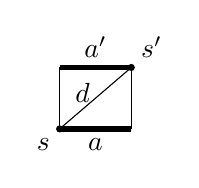
\begin{tikzpicture}[scale=.65]
\draw (0,0) rectangle (1.4,1.2);
\draw[line width=2pt] (0,0)--(1.4,0) (0,1.2)--(1.4,1.2);
\draw (0,0)--(1.4,1.2);
\fill (0,0) circle (2pt) (1.4,1.2) circle (2pt);
\node[below left] at (0,0) {$s$};
\node[above right] at (1.4,1.2) {$s'$};
\node[above] at (.7,1.2) {$a'$};
\node[below] at (.7,0) {$a$};
\node at (.45,.7) {$d$};
\end{tikzpicture}}}
tandis que $\underline{\omega}_Q$ s'identifie à
\deleted{l'ensemble} un ensemble de deux parties de $R$ (``$R^+$'' et ``$R^-$'')
complémentaires l'une de l'autre, et stables chacune par l'antipodisme
$\underline{a}$ (qui conserve l'orientation), ce qui fait que le choix d'un
élément de $R/\underline{a}$ définit canoniquement une orientation de $Q$,
\deleted{\unsure{un}} i.e. un des deux \deleted{\unsure{sous-ens.}} ens. de
repères $R',R''$.
Pour vérifier que à cette description d'une isom.
$C\wedge D\simeq\underline{\omega}_Q$ i.e. d'une relation
$\underline{\omega}_Q\wedge C\wedge D\simeq1$ correspond à
\deleted{\unsure{$\varpi\wedge c\wedge d=0$}}\inserted{$\varpi c d=1$},
il faut expliciter d'abord les conventions qui nous
\deleted{font} conduisent aux plongements
\[
 C\hookrightarrow V_S\setminus\{1,\underline{a}\}\subset\mathfrak{D},
 \qquad D\hookrightarrow V_A\setminus\{1,\underline{a}\}\subset\mathfrak{D},
 \qquad \underline{\omega}_Q\subset\mathfrak{D}^+\subset\mathfrak{D}
\]
Si $c$ est une \inserted{codiagonale i.e.} paire de côtés opposés du carré,
je vais lui associer l'autom. $g$ du carré qui fixe ces deux côtés
et qui échange les deux autres i.e. la symétrie p.r. à l'axe transversal.
De même, pour une diagonale, je lui associe la symétrie par rapport à cette
diagonale. Pour une orientation définie par un repère
\deleted{\unsure{ce}}
\figure{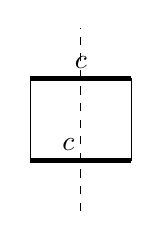
\begin{tikzpicture}[scale=.8]
\draw (0,0) rectangle (1.6,1.3);
\draw[line width=2pt] (0,0)--(1.6,0) (0,1.3)--(1.6,1.3);
\draw[dashed] (.8,-.8)--(.8,2.1);
\node[above] at (.8,1.3) {$c$};
\node[above] at (.6,0) {$c$};
\end{tikzpicture}
\qquad
\begin{tikzpicture}[scale=.8]
\draw[dashed] (0,0) rectangle (1.6,1.3);
\draw[dashed] (-.65,-.53)--(2.1,1.71);
\node[left] at (0,0) {$d$};
\node[above left] at (1.6,1.3) {$d$};
\end{tikzpicture}}

\scanpage{14}
% archive foliation: 13
\figure{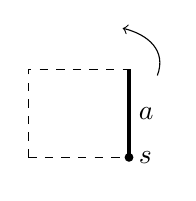
\begin{tikzpicture}[scale=.8]
\draw[dashed] (0,0)--(0,1.4)--(1.6,1.4);
\draw[dashed] (0,0)--(1.6,0);
\draw[line width=1.5pt] (1.6,0)--(1.6,1.4);
\fill (1.6,0) circle (2pt);
\node[right] at (1.6,0) {$s$};
\node[right] at (1.6,.7) {$a$};
\draw[->] (2.05,1.3) .. controls (2.2,1.7) and (1.9,1.95) .. (1.5,2.05);
\end{tikzpicture}}
je lui associe la rotation du carré qui transforme $s$ en le deuxième sommet
de $a$. On vérifie qu'avec ces conventions, la formule $\varpi cd=1$
est bien la formule qui exprime que $R_{\varpi}\subset R$ contient l'image
inverse par $R\mathbin{-}R/\underline{a}$ de l'élément $(c,d)$ de
$R/\underline{a}$.

Le fait que si on exprime la $=$ relation pour le carré dual, on semble
obtenir le résultat opposé, provient du fait que si on identifie le $=$
ensemble $R$ à l'ens. des repères de $Q$ \uline{et} de $Q^\circ$,
\deleted{\unsure{identifie}}\inserted{et} le $=$ groupe $\mathfrak{D}$ à
$\operatorname{Aut}Q$ \uline{et} à $\operatorname{Aut}(Q^\circ)$,
(ce qui n'est possible canoniquement que d'une seule façon
\inserted{raisonnable}, i.e. ce n'est pas une question de choix de
conventions\ldots) alors une $=$ \deleted{partie}\inserted{classe} $R'$ de $R$
\deleted{\unsure{comme}} (pour la relation d'équivalence de l'orientation),
considérée comme définissant une orientation de $Q$ \uline{et} une orientation
de $Q^\circ$, définit deux orientations \uline{opposées}, en ce sens que
les autom. de rotation qu'il définit via un repère $(s,a)$, suivant qu'il est
regardé comme un rep. de $Q$ ou un rep. de $Q^\circ$,
\unsure{sont} \uline{opposés} l'un de l'autre : transformer $s$ en $s'$ ou
$a$ en $a'$ se fait par deux rotations \uline{opposées}.
\figure{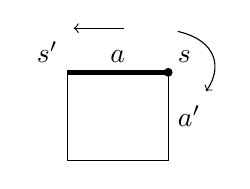
\begin{tikzpicture}[scale=.8]
\draw (0,0)--(0,1.4)--(1.6,1.4)--(1.6,0)--cycle;
\draw[line width=1.6pt] (0,1.4)--(1.6,1.4);
\fill (1.6,1.4) circle (2pt);
\node[above left] at (0,1.4) {$s'$};
\node[above right] at (1.6,1.4) {$s$};
\node[above] at (.8,1.4) {$a$};
\node[right] at (1.6,.7) {$a'$};
\draw[->] (.9,2.1)--(.1,2.1);
\draw[->] (1.75,2.05) .. controls (2.4,1.9) and (2.45,1.45) .. (2.2,1.1);
\end{tikzpicture}}

\scanpage{15}
\mspage{7}
Considérons le groupe $\mathfrak{D}$ en tant que groupe ``abstrait'', il est canoniquement extension de $\mathfrak{D}_{\mathrm{ab}}=W$ ($\simeq\mathbb{F}_2\times\mathbb{F}_2$ non canoniquement) par $\mathbb{F}_2$. Dans $\mathfrak{D}_{\mathrm{ab}}$ il y a un élément non nul distingué, \inserted{$\varpi$}, \deleted{\unsure{image inverse}}\inserted{dont l'image} inverse est l'ens $\underline{\omega}_Q$ des deux éléments d'ordre $4$ de $\mathfrak{D}$. On voit aisément que les deux autres éléments non nuls de $\mathfrak{D}_{\mathrm{ab}}$ sont interchangés par le groupe des autom. de $\mathfrak{D}$, on trouve donc
\diagram{\begin{tikzcd}[column sep=large]
1 \arrow[r] &
\underset{\substack{\text{autom. de l'ext. $\mathfrak{D}$ de}\\
\text{$W$ par $\mathbb{F}_2$ qui}\\
\text{induisent l'identité}\\
\text{dans $W$ et $\mathbb{F}_2$}}}{\check W}
\arrow[r] & \operatorname{Aut}\mathfrak{D} \arrow[r] &
\underbrace{\pm1}_{\substack{\text{interchange}\\
\text{les les deux}\\
\text{éléments de}\\
W\setminus\{0,\varpi\}}} \arrow[r,dash] & 1
\end{tikzcd}}
\margin{\uline{NB} on a en fait un iso. can. $\check W\simeq W$ ($\forall$ vectoriel de rg $2$ sur $\mathbb{F}_2$).}
$\operatorname{Aut}\mathfrak{D}$ est pr. semi-direct de $\pm1$ par $\check W$, $\pm1$ opérant par échange des $2$ éléments non \deleted{\unsure{distin.}} privilégiés de $\check W\simeq W$. Quand on tient compte que $\mathfrak{D}$ provient d'un carré, donc il y a choix d'un élément $\underline{c}$ de $W\setminus\{0,\varpi\}$ (correspondant \deleted{\unsure{aux}} à $C=\!V_S\setminus\{1,a\}$), l'autre élément étant $\underline{d}$ (correspondant à $D=V_A\setminus\{1,a\}$).
Les autom. de $\mathfrak{D}$ qui respectent cette structure forment le sous-groupe $\check W\simeq W$ de $\operatorname{Aut}\mathfrak{D}$, formé des autom. \inserted{d'ext.} qui induisent l'identité sur le quotient $W$. Ce sont aussi les autom. intérieurs, qui forment bien le groupe $W\simeq\mathfrak{D}/\underbrace{\{1,a\}}_{\text{centre}}$. (\unsure{Comme} l'hom $\mathfrak{D}\xrightarrow{\mathrm{int}}\operatorname{Aut}\mathfrak{D}$ n'est pas injectif), on voit que la donnée du groupe $\mathfrak{D}=\operatorname{Aut}_Q$ (qui revient à la donnée de $C$ et de $D$, cf plus bas)
\deleted{\unsure{revient à} $\mathfrak{D}=\mathbb{F}_2^C\mathbin{*_{\mathbb{F}_2}}\mathbb{F}_2^D$ \unsure{)}}
% archive foliation: 14

\scanpage{16}
ne peut suffire à reconstruire $Q$ à isom. unique près -- mais seulement $Q$ ``modulo antipodisme''. Considérons le carré épinglé $Q_0$, et le groupe de ses automorphismes
\[
\deleted{\mathfrak{D}_4}\quad D_4=\operatorname{Aut}(Q_0)
\]
avec la suite exacte canonique
\diagram{\begin{tikzcd}
1 \arrow[r] & \mathbb{F}_2 \arrow[r] & D_4 \arrow[r] & \mathbb{F}_2^2 \arrow[r,dash] & 1
\end{tikzcd}}
et la donnée de notre $\mathfrak{D}$ revient à celle d'un torseur sous $\mathbb{F}_2^2$ \inserted{le quotient de $D_4$} (i.e. de deux ens. à deux éléments (ce sont en fait $D$ et $C$, dans cet ordre\ldots)), tandis que celle d'un carré revient à la donnée d'un torseur sous $D_4$ lui-$=$.

On a une opération \inserted{(par autom. int.)} de $\mathfrak{D}^+$ sur $D$\inserted{$\hookrightarrow\mathfrak{D}^+$}, la donnée de $Q$ (correspondant au groupe d'autom $\mathfrak{D}$) \deleted{\unsure{nous}} revient à celle d'un relèvement de \deleted{\unsure{$\mathfrak{D}$}} l'opération \deleted{\unsure{induite de}} en \deleted{\unsure{les}} une opération \deleted{\unsure{sur}} transitive sur un ens. $S$, \inserted{(du \unsure{m.|même} gr. bien sûr $\mathfrak{D}$)} avec $S/\underline{a}\simeq D$.
Description duale via $C\hookrightarrow\mathfrak{D}^+$\ldots

\uline{Remarque.} Le groupe $\operatorname{Aut}(D_4)$ est isom. à $D_4$ (mais \uline{pas} via autom. intérieurs, bien sûr), ce qui implique qu'il y a \inserted{quand même} une équivalence de groupoïdes
\[
(\text{Carrés})\xrightarrow{\approx}(\text{groupes isom. à }D_4)
\]
(mais qui n'est \unsure{$\not=$} donnée par \deleted{\unsure{$\operatorname{Aut}_Q$}} $Q\mapsto\operatorname{Aut}(Q)$ !), qui mériterait d'être comprise\ldots
% archive foliation: 15

\scanpage{17}
\mspage{8}
Si $\mathfrak{D}$ est un groupe isomorphe à $D_4$, l'ens $S$ des éléments d'ordre $2$ \deleted{\unsure{non centraux}}\inserted{$\ne\underline{a}$ (où $\underline{a}$ est} l'unique élément central $\ne1$) \deleted{\unsure{est}} a quatre éléments, \deleted{\unsure{qui permet déjà de voir par quelle}} \inserted{sur lequel on a une involution} sans point \deleted{\unsure{fixe}} fixe par
\[
x\longmapsto x\unsure{\cdot|+}\underline{a}\underset{\mathrm{def}}{=}x'
\]
donc à $\mathfrak{D}$ correspond un carré $Q_{\mathfrak{D}}$, dont l'ens des sommets est $S$, et l'\deleted{\unsure{involution de}}\inserted{action de} l'antipodisme sur $S$ est l'involution précédente.
Mais le foncteur de groupoïdes $\mathfrak{D}\mapsto Q_{\mathfrak{D}}$
\[
(\text{groupes isom. à }D_4)\longrightarrow(\text{carrés combinatoires})
\]
est une équivalence de groupoïdes, car on reconstitue $\mathfrak{D}$ à partir de $(S,\underline{a}_S:\inserted{x\mapsto x'})$ \deleted{\unsure{prenant}}\inserted{par} la formule
\[
\mathfrak{D}=\left\{
\underbrace{x\in S,\ \underline{a}}_{\text{générateurs}}\ \middle|\
\underbrace{[x,y]}_{\substack{\text{commutateur}\\xyx^{-1}y^{-1}}}
=\underline{a}\ \text{si }y\ne x,x'
\right\}.
\]
\margin{\uline{NB} Si à un carré $Q$ on associe le groupe $\mathfrak{D}=\operatorname{Aut}(Q)$, puis le carré associé à ce groupe, on trouve le carré dont l'ens des sommets est $C\amalg D$, l'action de l'antipodisme dans \deleted{\unsure{chaque}} chacun d'eux $C$ et $D$, i.e. les diagonales sont $C$ et $D$. On trouve donc un carré avec diagonale \deleted{\unsure{privil.}}\inserted{distinguée}\ldots}

Si on part, pour décrire la structure de carré, de l'ens des sommets $S$, cette structure est exprimée par la donnée d'un ens. \inserted{$S$} à $4$ éléments -- i.e. d'un torseur sous un vectoriel $V_S$ de rang $2$ sur $\mathbb{F}_2$ -- et d'une \deleted{\unsure{f}} involution ss pt fixes de $S$, i.e. d'un $\underline{a}_S\in V_S^*$ \deleted{Mais \unsure{ce}}\inserted{(\unsure{i.e.} une} \deleted{\unsure{$V=V_S^*$}} partition de type $(2,2)$ de $S$). Mais pour
% archive foliation: 16

\scanpage{18}
un vectoriel \inserted{$V$} de rg $2$ sur $\mathbb{F}_2$, la donnée d'un $a\in V^*$ revient à la donnée d'une partie de $V$ qui soit une base (savoir $V^*\setminus\{a\}$); donc la donnée d'un \inserted{couple $(V,a)$ d'un} vectoriel $V$ de rg $2$ sur $\mathbb{F}_2$, et d'un élément \inserted{$a$} de $V^*$, revient à la donnée d'un ens. $C$ à deux éléments, par $V\simeq\mathbb{F}_2^C$, $a$ l'élément diagonal de $\mathbb{F}_2^C$.
Ainsi, la donnée d'un carré $Q$ \deleted{\unsure{via ses sommets}} (via l'ens des sommets) équivaut à celle d'un couple $(C,S)$, où $C$ \deleted{\unsure{est $\mathbb{F}_2$}} est un ens. à deux éléments, et $S$ est un torseur sous $\mathbb{F}_2^C$. Mais la donnée d'un tel torseur revient à celle d'une famille de $\mathbb{F}_2$-torseurs indexée par $C$, i.e. d'une application de degré $2$
\[
A\longrightarrow C,
\]
\unsure{a|à} quatre éléments, et est muni d'une involution sans pts fixes (qui donne le passage au quotient vers $C$), par la formule
\[
S\simeq\prod_{c\in C}\deleted{\mathbb{F}_2}A_c
=\text{Ens des sections de $A$ sur $C$}
\]
qui donne en même temps un plongement
\[
S\hookrightarrow\unsure{\mathcal{P}_2(A)|\mathcal{P}_2(A)_a}
\]
d'où la relation d'incidence entre $S$ et $A$\ldots
\margin{ici les deux $A_c$ ($c\in C$) \unsure{sont} \deleted{\unsure{naturellement}} \unsure{les} \uline{quotients} de $S$, par les relations d'équivalence définies resp. par \deleted{les} \inserted{les $2$ élémts} \unsure{éléments} \inserted{$c\in C$} \deleted{\unsure{deux}} de $V^*$ (considérés comme involutions ss pt fixes de $S$). Mais je préfère ici prendre la construction inverse, en \deleted{identifiant} introduisant \unsure{deux} $A_c$ et $A_{c'}$.}
% archive foliation: 17

\scanpage{19}
\mspage{9}
Dualement, \deleted{\unsure{$A$ est de}} la donnée d'un carré-arêtes $A$ s'interprète comme la donnée d'un torseur sous un groupe $\mathbb{F}_2^D$, ce qui équivaut à la donnée d'une famille de \inserted{$\mathbb{F}_2$-}torseurs $(S_d)_{d\in D}$, \deleted{\unsure{indexée par un ens. $S$}}
\[
A\simeq\prod_{d\in D}S_d\qquad(\simeq\text{sections de $S$ sur $D$})
\]
-- la donnée de cette famille équivaut à la donnée d'un ensemble (à quatre éléments) $S$ et d'une application de degré $2$
\[
S\longrightarrow D
\]
qui avec la formule précédente donne
\[
A\hookrightarrow\mathcal{P}_2(S)
\]
et la relation d'incidence entre $S$ et $A$\ldots

\uline{Formulaire} On a, pour un carré $Q$, les trois ensembles à deux éléments
\[
\underset{\text{codiagonales}}{C},\quad
\underset{\text{diagonales}}{D},\quad
\underset{\text{orientations}}{\underline{\omega}}
\]
plus les deux paquets de deux ens. à deux éléments (ou $4$ autres ens. à deux éléments)
\[
\begin{array}{cc}
S\xrightarrow{\mathrm{deg.}\,2}D,&A\xrightarrow{\mathrm{deg.}\,2}C\\
(D\simeq S/\underline{a}_S).&(C\simeq A/\underline{a}_A)
\end{array}
\]
On a le formulaire d'iso. can.
% archive foliation: 18

\scanpage{20}
\[
\boxed{\begin{gathered}
(1)\qquad \underline{\omega}_S\simeq C,\quad\underline{\omega}_A\simeq D\\
(2)\qquad \underline{\omega}\wedge C\wedge D\simeq\underline{1}_{\mathbb{F}_2}
\quad\text{i.e.}\quad
\left\{\begin{array}{l}
\underline{\omega}\simeq C\wedge D\\
C\simeq D\wedge\underline{\omega}\\
D\simeq\underline{\omega}\wedge C
\end{array}\right.\\
(3)\qquad D\simeq S/\underline{a}_S,\quad C\simeq A/\underline{a}_A\\
(4)\qquad S\simeq\prod_{c\in C}A_c,\quad A\simeq\prod_{d\in D}S_d\\
(5)\qquad D\simeq\bigwedge_{c\in C}A_c,\quad C\simeq\bigwedge_{d\in D}S_d\\
\text{ces \inserted{deux} dernières relations provenant de}\\
\underline{\omega}\simeq\left(\bigwedge_{c\in C}A_c\right)\wedge C
\quad\text{d'où}\quad
\underbrace{\underline{\omega}\wedge C}_{D\text{ par }(2)}
\simeq\bigwedge_{c\in C}A_c .
\end{gathered}}
\]

3. Complément sur les \unsure{$2$|$3$}-ss-groupes \deleted{de Sylow} d'un groupe \inserted{$G=$}$\unsure{\mathcal{G}_I|\mathfrak{S}_I}$ ($\operatorname{card}I=4$).
\margin{À commencer par les \unsure{$2$|$3$}-sous-groupes de Sylow.}

Soit $V$ le sous-groupe distingué $\simeq\mathbb{F}_2^2$, de sorte que $V^*\simeq\mathcal{P}_{2,2}(I)$. On a
\diagram{\begin{tikzcd}[column sep=huge,row sep=huge]
\substack{\text{Ens des structures}\\\text{de carré sur }Q}\simeq V^* \arrow[rr,leftrightarrow,"\sim"] \arrow[dr,leftrightarrow,"2"'] &&
\substack{\text{Sous-groupes cycliques }\mathfrak{D}^+\\\text{d'ordre $4$ de $G$}}
\arrow[dl,leftrightarrow,"1"]\\
& \substack{\unsure{2|3}\text{-sous-groupes}\\\text{de Sylow de }G} &
\end{tikzcd}}
\margin{(à $Q$ correspond à $\mathfrak{D}^+$, qui correspond à $\operatorname{Aut}Q=\mathfrak{D}$)}
\margin{pour tt ss gr. cyclique $\mathfrak{D}^+$ il a un unique él. d'ordre $2$, qui est dans $V^*$, et $\mathfrak{D}^+$ en est le centralisateur}
\margin{pour $\forall$ sous-groupe de Sylow $\mathfrak{D}$, il y a un unique élément $x$ central $\ne1$, et celui-ci est dans $V^*$, et $\mathfrak{D}$ est le normalisateur ou centralisateur de $x$}
\margin{tout sous-groupe de Sylow $\mathfrak{D}$ a un unique ss-groupe cyclique d'ordre $4$, $\mathfrak{D}^+$, et il en est le normalisateur}
% archive foliation: 19

\scanpage{21}
\mspage{10}
Quels sont les sous-groupes de \inserted{$G=$}$\unsure{\mathcal{G}_I|\mathfrak{S}_I}$ \deleted{\unsure{$t$}}, $\ne e$ et $\unsure{\mathcal{G}_I|\mathfrak{S}_I}$ ?

A) Sous-groupes d'ordre une puissance de $2$, i.e. contenus dans un $2$-sous-groupe de Sylow $\mathfrak{D}$.

\deleted{Sous-groupes cycliques \unsure{correspondant aux}}

1) Ss-groupes d'ordre $2$, correspondant aux éléments d'ordre $2$ :

a) les \inserted{trois} éléments de $V^*$, qui forment une orbite sous $\operatorname{Int}G$.
\margin{$3$\qquad$V^*$}

b) les six transpositions ou réflexions, qui forment une autre orbite sous $\operatorname{Int}G$, et se groupent en trois paquets (indexés par $V^*$) de deux, par la relation $\tau\tau'\in V^*$, ou par celle d'être contenus dans un \inserted{$=2$-}ss-groupe de Sylow.
\margin{$6$\qquad$\widetilde{V}^*$}
\margin{i.e. $\tau,\tau'$ ont $=$ image dans $\unsure{\mathcal{G}_J|\mathfrak{S}_J}$}

\deleted{\unsure{cycliques}}
2) Sous-groupes d'ordre $4$

c) \inserted{les trois} Sous-groupes cycliques d'ordre $4$, qui \deleted{correspondant à \unsure{chacun des trois}}\inserted{correspondent $1$-$1$ aux trois} sous-groupes de Sylow i.e. les trois structures de carré sur $I$.
\margin{$3$\qquad$V^*$}

d) Sous-groupes non cycliques d'ordre $4$, donc isom. à $\mathbb{F}_2\times\mathbb{F}_2$ -- il y a d'abord $V^*$
\margin{$1$}

e) puis ceux qui ne sont pas distingués, chacun contenu dans un unique ss-groupe de Sylow, dans lequel il y en \deleted{\unsure{deux}}\inserted{un} comme ça, \inserted{(en plus de $V$, \unsure{qui en a quatre|qui en est un autre})}, donc il y en a en tout \deleted{six}\inserted{trois} sous-groupes \deleted{$\mathbb{F}_2\times\mathbb{F}_2$} $(2,2)$ non distingués, qui \deleted{forment \uuline{deux}}\inserted{forment une} \unsure{classe} de conjugaison \deleted{distinctes, de trois éléments savoir les $V_S\in\mathfrak{D}$ et les $V_A$, correspondants}
\margin{$3$\qquad$V^*$}

3) Sous-groupes d'ordre $8$ -- ce sont les

f) trois sous-groupes de Sylow de $G$
\margin{$3$\qquad$V^*$}
% archive foliation: 20

\scanpage{22}
\uline{B)} Considérons ensuite les sous-groupes \inserted{de $G$} d'ordre multiple de $3$, donc d'ordre $3$, $6$ ou $12$.

g) Sous-groupes d'ordre $3$, ce sont les $4$ $3$-sous-groupes de Sylow, indexés par les éléments de $I$
\margin{$I\quad4$}

h) Les sous-groupes d'ordre $6$ ne sont pas cycliques (il n'y a pas d'élément d'ordre $6$) donc sont isomorphes à $D_3$, \deleted{\unsure{ce}} ce sont les quatre stabilisateurs des pts de $I$, i.e. les normalisateurs des $3$-sous-groupes de Sylow
\margin{$I\quad4$}

i) Il y a un seul sous-groupe d'ordre $12$ i.e. d'indice $2$, du seul fait que $\deleted{\unsure{G_2|\mathbb{F}_2}}\unsure{\mathcal{G}_{\mathrm{ab}}|\mathfrak{S}_{\mathrm{ab}}}\simeq\{\pm1\}$, et c'est $G^+\simeq\unsure{\mathcal{G}_I^+|\mathfrak{S}_I^+}$, ss-groupe \uline{alterné} de $\unsure{\mathcal{G}_I|\mathfrak{S}_I}$
\margin{$1$}

Il y a donc \inserted{exactement} $19$ sous-groupes qui sont des deux-sous-groupes, $\ne e$, se répartissant en \uline{six} classes de conjugaison (\deleted{\unsure{bien}}\inserted{correspondant à} $6$ classes d'isomorphismes d'espaces homogènes sous $G$), et $9$ sous-groupes \inserted{$\ne G$} qui sont d'ordre multiple de $3$, se répartissant en trois autres classes de conjugaison. Cela fait en tout $28$ sous-groupes, donc $30$ en comptant $\{e\}$ et $G$, se répartissant en $9$ classes de conjugaison (comp. $11$ en comptant $\{e\}$ et $G$), qui correspondent à autant de classes d'isomorphie d'espaces homogènes sous $G$.
\margin{Pour bien faire, il faudrait les inclure dans un diagramme d'inclusions, ou diag. de morphismes d'espaces homogènes.}
% archive foliation: 21

\scanpage{23}
\mspage{11}
4. \uline{Relations avec le cube orienté}

Si $I$ est un ens. à $4$ éléments, $J\simeq\mathcal{P}_{2,2}(I)\simeq V_I^*$ l'ens à trois éléments associé, on considère l'application de degré $2$
\diagram{\begin{tikzcd}
(*)\quad \operatorname{Circ}(I) \arrow[r] & J\\
\substack{\text{ens des permutations}\\\text{circulaires sur }I} &\\
u \arrow[r,mapsto] & u^2
\end{tikzcd}}
[NB On a aussi l'application de degré $2$
\diagram{\begin{tikzcd}
\mathcal{P}_2(I) \arrow[r] & J\\
A \arrow[r,mapsto] & \{A,I\setminus A\}
\end{tikzcd}}
$\simeq$ ens. des ``\unsure{dicompositions|décompositions} de $I$'' (ou ``réflexions'')
\[
\text{ou }\forall\tau\ \text{réflexion},\
\exists!\tau'\ \text{réflexion telle que }\tau\tau'\in V^*.
\]
ce sont vraiment des revêtements de nature distincte, les espaces homogènes \inserted{sous $G$} $\operatorname{Circ}(I)$ et $\mathcal{P}_2(I)$ n'étant pas \unsure{$\tilde m$} isomorphes (le stabilisateur d'un élément de $\operatorname{Circ}$ est $\simeq\mathbb{Z}/4\mathbb{Z}$, celui d'un élément de $\mathcal{P}_2(I)$ est $\simeq\mathbb{F}_2\times\mathbb{F}_2$) -- c'est le premier des deux, \inserted{\unsure{i.e.} $\operatorname{Circ}(I)$}, qui peut s'interpréter comme \deleted{l'application}\inserted{l'ens des} \deleted{\unsure{de $\varphi$}}\inserted{des} faces d'un cube\ldots].

L'application de degré $2$ $(*)$ définit un cube \inserted{comb.} dont l'ens. des faces est $\operatorname{Circ}(I)$, \inserted{avec l'antipodisme $u\mapsto u^{-1}$}, l'ens des \deleted{\unsure{sommets}}\inserted{arêtes} (resp. des sommets) \deleted{\unsure{est}} \inserted{est} l'ens des $12$ sections partielles \deleted{\unsure{tous}} sur des parties de card. $2$ de $J$ (resp. des \deleted{\unsure{six}} $8$ sections de $\operatorname{Circ}(I)$ sur $J$), l'incidence entre \deleted{\unsure{les faces}}\inserted{éléments de dim. $2,1,0$} étant le prolongement des sections partielles. \deleted{À \unsure{tout}} Il y aurait
\margin{Bien sûr, $G$ opère sur le cube par isomorphismes.}
% archive foliation: 22

\scanpage{24}
lieu d'expliciter

a) la correspondance entre \inserted{les $8$} sommets du cube, et les \inserted{$8$} éléments d'ordre $3$ de $G$ (``rotations-sommets'')

b) \deleted{les éléments}\inserted{la corr.} entre les $6$ paires d'arêtes antipodiques du cube, et les $6$ \deleted{\unsure{réflexions}} réflexions de $G=\unsure{\mathcal{G}_I|\mathfrak{S}_I}$

c) la corr. entre les $6$ \deleted{éléments de $\operatorname{Circ}(I)$, et}\inserted{faces du cube, et} les \deleted{$6$ \unsure{deux éléments de $G$}}\inserted{permutations circulaires} (él. d'ordre $4$ de $G\simeq\operatorname{Aut}^+(\text{Cube})$) correspondants,

et de décrire également une \uline{orientation canonique} du cube, ou ce qui revient au $=$, une \deleted{trivialisation} iso.
\[
\underset{\substack{\Vert\mathrm{def}\\\underline{\omega}_J(\simeq\underline{\omega}_I)}}
{\underline{\omega}_{\unsure{C|Q}}}
\simeq \bigwedge_{i\in J}
\underset{\substack{\text{ens des deux \deleted{\unsure{éléments}}\inserted{autom.} d'ordre $4$}\\
\text{dans la structure carré}\\
Q_i\text{ définie par }i\in J\\
\text{i.e. ens des deux orientations}\\
\text{de }Q_i.}}{\underline{\omega}_i}
\]

Comme on a
\[
\underline{\omega}_i\simeq
\underset{\substack{\text{ens. des deux}\\\text{codiagonales de }Q_i}}
{\underline{\omega}}\wedge
\underset{\substack{\text{ens des diag.}\\
\text{pour le carré }Q_i,\ \text{i.e. }D_i=
I/\underset{\text{translation indiquée par }i}{\underline{a}_i}}}{D_i}
\]
la formule \deleted{\unsure{antérieure}} s'écrit aussi
\[
\underset{\substack{\text{\unsure{torseur}}\\\text{sous }\mathbb{F}_2^J}}
{\bigwedge_{i\in J}D_i}\simeq\underline{1}
\]
Or on a \deleted{la suite exacte} l'inclusion
\diagram{\begin{array}{ccc}
I&\hookrightarrow&\prod_{i\in J}D_i\\
\substack{\text{torseur}\\\text{sous }V_J(\mathbb{F}_2)}
&\subset&
\substack{\text{torseur sous}\\\mathbb{F}_2^J}
\end{array}}
% archive foliation: 23

\scanpage{25}
\mspage{12}
qui fait une restriction du groupe structural à $V_J(\mathbb{F}_2)$, d'où $\bigwedge_{i\in J}D_i\simeq\underline{1}$, OK.

Il y aurait lieu aussi d'interpréter les $10$ classes d'isomorphie d'espaces homogènes $\ne(1)$ sous $G\simeq\operatorname{Aut}(\text{Cube})$ (correspondant à des \deleted{\unsure{deux}} sous-groupes d'isotropie $\ne G$, définis à conjugaison près) en termes d'\deleted{\unsure{objets}} éléments de structure associés au cube (les sommets, arêtes, faces, ou lesdits mod antipodisme -- i.e. sur le cube \unsure{gauche} -- ou \deleted{\unsure{repères de paires}}\inserted{repères} d'arêtes -- ce qui en fait déjà sept \inserted{ens.} de cardinaux $8,12,6,\ 4,6,3,\ 24$.
Il y en a un de cardinal $2$, quotient de l'ens des sommets (correspondant à l'ens. $\underline{\omega}_I$), un autre d'ordre $12$ correspondant aux diagonales des faces \inserted{(ou codiagonales, si on préfère)} (les stabilisateurs, \deleted{\unsure{de ces éléments d'ordre}}\inserted{correspondent aux él.} d'ordre $2$ de $G$ qui ne sont pas dans $V$), enfin un troisième qui est formé des paires d'éléments distincts de $J$ (i.e. repères de $J$), $J$ étant interprété comme l'ens des ``directions de faces'' \deleted{\unsure{(=}} (ens des faces/antipodisme) ou des directions d'arêtes. Le compte y est !
\margin{position relative de deux sommets à dist. comb. $1$, ou encore de deux arêtes à dist. comb. \unsure{$2$}, \deleted{ou à dist. \unsure{$2$}}}
\deleted{\unsure{$\mathcal{E}$}}
% archive foliation: 24

\scanpage{26}
5. Modules libres de rang $2$ sur $\Lambda=\mathbb{Z}/4\mathbb{Z}$.

Soit $M$ un tel module, et soit
\[
(1)\qquad M_0=M/2M=M\otimes_\Lambda\mathbb{F}_2
\]
qui est un vectoriel de rang $2$ sur $\mathbb{F}_2$. Soit $J=M_0^*$, on utilise la notation indicielle pour les éléments de $M_0^*$, notés $x_i$ ($i\in J$). \deleted{Pour tout $i\in J$, soit}

On a une suite exacte de \deleted{groupes \unsure{comm.}}\inserted{$\Lambda$-modules}.
\diagram{\begin{tikzcd}
(2)\quad0 \arrow[r,dash] & M_0 \arrow[r] & M \arrow[r,"\mathrm{can}"] & M_0 \arrow[r] & 0\\
& M \arrow[u,dotted,"\mathrm{can}"'] \arrow[ur,dotted,"2"'] &&&
\end{tikzcd}}
donc $M$ apparaît comme extension de $M_0$ par $M_0$ (en tant que $\Lambda$-module). Pour $\forall x\in M_0$, soit $M_x$ son image inverse dans $M$, qui est un torseur sous $M_0$ (i.e. un ens. à quatre éléments \inserted{$M_x$}, muni d'un iso. $M_0\simeq V_{M_x}$).

On posera, pour $i\in J$
\[
(3)\qquad
\left\{\begin{array}{l}
M_i=M_{x_i}=\deleted{\text{\unsure{image inverse de $\{x_i\}$}}}
\inserted{\text{fibre de $M$ sur }}x_i\in M_0,\ M_0\text{-torseur}\\
M_J=\prod_{i\in J}M_i,\ \text{un torseur sous }\deleted{\unsure{\mathbb{F}_2}}M_0^J.
\end{array}\right.
\]
Comme on
\[
(4)\qquad\sum_{i\in J}x_i=0
\]
la structure de groupe sur $M$ donne un iso. can.
\[
(6)\qquad\bigwedge_{i\in J}M_i=0
\]
en d'autres termes, introduisant
\[
(7)\qquad V_J(M_0)=\left\{(\unsure{\xi_i|\bar{x}_i})_{i\in J}\in M_0^J\mid\sum\xi_i=0\right\}
\]
s'insérant dans la suite exacte
\diagram{\begin{tikzcd}
(8)\quad0 \arrow[r,dash] & V_J(M_0) \arrow[r,dash] & M_0^J \arrow[r,dash,"\text{somme}"'] & M_0 \arrow[r,dash] & 0,
\end{tikzcd}}
le torseur $M_J$ sur $M_0^J$ provient canoniquement d'un torseur sous $V_J(M_0)$, que je note $P_M$,
% archive foliation: 25

\scanpage{27}
\mspage{\textcircled{13}}
De façon précise, \inserted{la donnée} des \inserted{$M_0$-torseurs} $M_i$ et \inserted{de} l'isom. can. $6$ revient à la donnée du torseur $P_M$ sous $V_J(M_0)$, avec
\[
(9)\qquad M_i\simeq P_M\wedge_{M_0^J}(M_0,\operatorname{pr}_i)
\qquad\text{pour }i\in J
\]
où $\operatorname{pr}_i:M_0^J\mathbin{-}M_0$ la projection d'indice $i\in J$.

Notons qu'on a des iso. canoniques (valables pour $\forall$ vectoriel de rang $2$ sur $\mathbb{F}_2$)
\[
(10)\qquad
\operatorname{End}(M_0)\simeq V_J(M_0)\xrightarrow{\sim}M_0\otimes M_0
\simeq M_0\oplus\mathbb{F}_2^{\underline{\omega}_{M_0}}
\]
\[
\underline{\omega}_{M_0}\simeq\underline{\omega}
(\underbrace{M_0^*}_{J})\quad\text{ens des orientations de }J.
\]
\margin{\uline{NB} Pour $\forall$ vectoriel $W$ sur $\mathbb{F}_2$ on a
\[
(11)\qquad\operatorname{Hom}_{\mathbb{F}_2}(M_0,W)\simeq V_J(W)
\]
Car $M_0\simeq\mathbb{F}_2^J/\mathbb{F}_2\text{ diag}$}
\diagram{\begin{tikzcd}
(12)\quad\operatorname{End}(M_0) \arrow[r,"\sim"] & V_J(M_0)\\
u \arrow[r,mapsto] &(u(x_i))_{i\in J}
\end{tikzcd}}
\[
\operatorname{End}(M_0)\simeq M_0^\vee\otimes M_0\simeq M_0\otimes M_0
\quad\text{car }M_0^\vee\simeq M_0
\]
(valable pour $\forall$ vect. de rang $2$ sur $\mathbb{F}_2$)

\diagram{\begin{tikzcd}
(13)\quad M_0 \arrow[r,hook] & \operatorname{End}(M_0)\\
M_0^* \arrow[u,phantom,"\cup" description] \arrow[r,hook] &
\operatorname{Aut}(M_0)\simeq\unsure{\mathcal{G}_J|\mathfrak{S}_J}
\arrow[u,phantom,"\cup" description]
\end{tikzcd}}
\[
x_i\longmapsto\deleted{\text{transposition}}\inserted{\sigma_i}
\quad\text{réflexion de $M_0$ qui fixe $x_i$}
\]
(donc \deleted{\unsure{qui est}}\inserted{transposition} des $x_j$ et $x_k$)
[\uline{NB} Comme $\sum_{i\in J}\sigma_i=0$, cela correspond à hom
$M_0\longrightarrow\operatorname{End}(M_0)$]

\diagram{\begin{tikzcd}
(14)\quad\mathbb{F}_2^{\underline{\omega}_{M_0}} \arrow[r,hook] &
\operatorname{End}(M_0)\\
\underline{\omega}_{M_0} \arrow[u,phantom,"\cup" description] \arrow[r,hook,"\mathrm{can}"] &
\operatorname{Aut}(M_0)\simeq\unsure{\mathcal{G}_J|\mathfrak{S}_J}
\arrow[u,phantom,"\cup" description]\\
\underline{\omega}_J
\simeq\unsure{\mathcal{G}_J^+|\mathfrak{S}_J^+}\setminus\{\operatorname{id}_J\}
\arrow[u,phantom,"\Vert" description] &
\end{tikzcd}}
\margin{\uline{NB} \uline{On a} -- si $\rho\in\underline{\omega}$,
$\rho'\underset{\mathrm{def}}{=}\rho^{-1}$
\[
\rho+\rho'+\unsure{1}\operatorname{id}=0
\]
i.e. $\rho+\rho'=\operatorname{id}_{M_0}$.}
i.e. l'hom $\mathbb{F}_2^{\underline{\omega}}\hookrightarrow\operatorname{End}(M_0)$ applique $1$ sur $1$.

Si $i,j\in J$, $i\ne j$, alors $\sigma_i,\sigma_j,\rho,\rho'\in\operatorname{End}(M_0)$ sont lin. indépendants sur $\mathbb{F}_2$ donc forment une base, \deleted{\unsure{de}} dès que $x_i,x_j$ en forment une de $M_0$, et $\rho,\rho'$ de $\mathbb{F}_2^{\underline{\omega}}$\ldots
% archive foliation: 26

\scanpage{28}
On a
\[
(15)\quad\left\{\begin{gathered}
M_0\text{ et }\mathbb{F}_2^{\underline{\omega}}
\text{ sont orthogonaux l'un de l'autre}\\
\text{dans }\uline{\operatorname{End}}(M_0)\text{ pour la forme }\operatorname{Tr}(uv)
\end{gathered}\right.
\]
\[
(16)\quad\deleted{\unsure{\mathbb{F}_2}}\ 
\underset{\operatorname{Ker}(\operatorname{End}(M_0)\xrightarrow{\mathrm{tr}}\mathbb{F}_2)}
{\mathfrak{sl}(M_0)}
=M_0\oplus\mathbb{F}_2\operatorname{id}_{M_0}
\]
\[
(17)\quad\mathbb{F}_2^{\underline{\omega}}\cap
\mathfrak{sl}(M_0)
\simeq\mathbb{F}_2\cdot\operatorname{id}_{M_0}\quad\ldots\qquad]
\]
Ainsi, la donnée d'un torseur $P_M$ sous \inserted{$V_J(M_0)\simeq$}$\operatorname{End}(M_0)$\deleted{\unsure{$a$}}, équivaut à celle d'un couple de torseurs, \deleted{sur} l'un sous $M_0$, l'autre sous $\mathbb{F}_2^{\underline{\omega}}$, soient $I_M$ et $S_M$.

\uline{Théorème} Le foncteur $M\mapsto(M_0,I_M,S_M)$
\diagram{\begin{tikzcd}
(18)\quad\substack{\mathbb{Z}/4\mathbb{Z}\text{-modules}\\\text{libres de rang }2}
\arrow[r] & \text{triplets }(M_0,I_{\deleted{M}},S_{\deleted{M}})
\end{tikzcd}}
\deleted{où $M_0$ un vect. de rg $2$}
avec
\[
\left\{\begin{array}{l}
M_0\text{ vect. de rg }2\text{ sur }\mathbb{F}_2\\
I\quad M_0\text{-torseur}\\
S\quad\text{torseur sous }\mathbb{F}_2^{\underline{\omega}(M_0)}
\end{array}\right.
\]
est une équivalence de groupoïdes.

\margin{Équivalent essentiellement à l'isomorphisme
\[
\operatorname{GL}(2,\mathbb{Z}/4\mathbb{Z})
\simeq\operatorname{GL}(2,\mathbb{F}_2)\cdot M_2(\mathbb{F}_2)
\]
(produit $\frac12$ direct), plus l'isomorphisme de $\unsure{\mathcal{G}_3|\mathfrak{S}_3}$-modules ($\unsure{\mathcal{G}_3|\mathfrak{S}_3}\simeq\operatorname{GL}(2,\mathbb{F}_2)$)
\[
M_2(\mathbb{F}_2)\simeq\mathbb{F}_2^2\times\mathbb{F}_2^{\underline{\omega}_0},
\]
où $\operatorname{GL}(2,\mathbb{F}_2)$ opère sur $\mathbb{F}_2^2$ tautologiquement, et sur $\mathbb{F}_2^{\underline{\omega}_0}$ via op. sur $\underline{\omega}_0$ par signature\ldots On a l'inclusion
\[
\operatorname{SL}(2,\mathbb{Z}/4\mathbb{Z})
\unsure{\subset|=}\operatorname{GL}(2,\mathbb{F}_2)\cdot
\deleted{\unsure{M_2(\mathbb{F}_2)}}
\]
\deleted{\unsure{$\operatorname{GL}(2,\mathbb{F}_2)\ltimes\mathbb{F}_2^2\times\mathbb{F}_2$}}
\[
\{g\cdot u\in\unsure{\mathcal{G}_3|\mathfrak{S}_3}\cdot M_2(\mathbb{F}_2)
\mid\operatorname{sg}(g)\underline{e}(\operatorname{Tr}u)=1\}
\]
où $\underline{e}:\deleted{\unsure{\mathbb{F}_2}}\mathbb{F}_2
\xrightarrow{\sim}\{\pm1\}$.}

\uline{Corollaire} On a un isom. de suites exactes canoniques ($\forall M$ libre de rg $2$ sur $\Lambda=\mathbb{Z}/4\mathbb{Z}$)
\diagram{\begin{tikzcd}
1\arrow[r,dash]&\operatorname{End}_{\mathbb{F}_2}(M_0)\arrow[r]&
\operatorname{GL}(M)\arrow[r]&
\operatorname{GL}(M_0)\simeq\unsure{\mathcal{G}_J|\mathfrak{S}_J}\arrow[r,dash]&1\\
(19)\quad1\arrow[r,dash]&
M_0\times\mathbb{F}_2^{\underline{\omega}}\arrow[u,"\sim"]\arrow[r]&
\operatorname{Aut}(M_0,I_M,S_M)\arrow[u,"\sim"]\arrow[r]&
\operatorname{GL}(M_0)\arrow[u,equal]\arrow[r,dash]&1.
\end{tikzcd}}
Ici l'hom $\operatorname{End}(M_0)\longrightarrow\operatorname{GL}(M)$ est donné par la condition que le composé avec l'hom $\operatorname{End}_\Lambda(M)\longrightarrow\operatorname{End}_{\mathbb{F}_2}(M_0)$ soit donné par
\[
u\longmapsto\operatorname{id}_M+2u.
\]
% archive foliation: 27

\scanpage{29}
\mspage{14}
% archive foliation: 28

La donnée de $(M_0,I)$ équivaut, par le §1, à la donnée d'un ens. à quatre éléments $I$, on aura $M_0\simeq V_I$, $M_0^*\simeq\mathcal P_{2,2}(I)$. \deleted{\unsure{Pour}} \inserted{D'autre} part, \unsure{\deleted{la donnée d'un}|\uline{la donnée d'un}} ens. à deux éléments $C$, et d'un torseur $S$ sous $\mathbb{F}_2^C$, équivaut à la donnée d'un carré $Q$, $S$ étant l'ens. des sommets de $Q$, $C$ l'ens de ses codiagonales.

Donc le \deleted{catégorie} \inserted{gr.ïde} du deuxième mb de (18) est équivalent à celui des triples $(I,Q;k)$, où $I$ est un ens à quatre éléments, $Q$ un carré, et $k$ un isom.
\[
(20)\qquad k:\underset{\substack{\text{ens des}\\\text{orientations}\\\text{de }I}}{\underline{\omega}(I)}
\simeq
\underset{\substack{\text{ens. des}\\\text{codiagonales}\\\text{de }Q}}{C(Q)}.
\]

On trouve donc

\uline{Corollaire 2} On a une équivalence can. de groupoïdes
\[
(21)\qquad
\underset{\mathbb{Z}/4\mathbb{Z}}{\underline{\Lambda}}\text{-modules libres de rg }2
\xrightarrow{\approx}
\text{triplets }(I,Q,k),\ \text{où}
\quad
\left\{
\begin{array}{l}
I\ \text{ens. à 4 éléments}\\
Q\ \text{carré combinatoire}\\
k:\underline{\omega}(I)\simeq C(Q).
\end{array}
\right.
\]

\uline{Corollaire 3} Si $M$ est associé à $I,Q$, on a un diagramme cartésien canonique
\[
(22)\qquad
\diagram{\begin{tikzcd}
& GL_\Lambda(M)\arrow[dl]\arrow[dr]&\\
\unsure{\mathcal{G}_I|\mathfrak S_I}\arrow[dr,"\mathrm{sg}"']&&\mathfrak D_Q\arrow[dl,"\chi_C\ (\text{opération sur l'ens des codiagonales})"]\\
&\{\pm1\}&
\end{tikzcd}}
\]

\scanpage{30}
% archive foliation: 29

s'insérant dans le diagramme de suites exactes (auquel il donne naissance)
\[
(23)\qquad
\diagram{\begin{tikzcd}[column sep=small,row sep=small]
&&&1\arrow[d]&&&\\
&&&\unsure{\mathcal{G}_I^+|\mathfrak S_I^+}\times\mathbb{F}_2^{\underline\omega}
\arrow[dl,"\mathrm{pr}_1"']\arrow[dr,"\mathrm{pr}_2"]\arrow[dd]&&&\\
&1\arrow[r]&\unsure{\mathcal{G}_I^+|\mathfrak S_I^+}\arrow[dl,Rightarrow]\arrow[dr]&&
\mathbb{F}_2^{\underline\omega}\arrow[dl]\arrow[dr,Rightarrow]&1\arrow[l]&\\
1\arrow[r]&\unsure{\mathcal{G}_I^+|\mathfrak S_I^+}\arrow[dr]&&GL_\Lambda(M)\arrow[dl]\arrow[dr]\arrow[dd,"\text{cart}"']&&
\mathbb{F}_2^{\underline\omega}\simeq V_{S_Q}\arrow[dl]&1\arrow[l]\\
&&\unsure{\mathcal{G}_I|\mathfrak S_I}\arrow[dl]\arrow[dr,"\mathrm{sg}"']&&
\mathfrak D_Q\arrow[dl,"\chi_C"]\arrow[dr]&&\\
&1&&\{\pm1\}\arrow[dl]\arrow[d,dash]\arrow[dr]&&1&\\
&&1&1&1&&
\end{tikzcd}}
\]

\uline{Proposition} Le \inserted{noyau $(\simeq\unsure{\mathcal{G}_I^+|\mathfrak S_I^+})$ de l'}hom. canonique $GL_\Lambda(M)\longrightarrow\mathfrak D_Q$
\deleted{induit un iso} est aussi égal au groupe des commutateurs du sous-groupe \inserted{distingué} $SL_\Lambda(M)$ d'indice $2$ de $GL_\Lambda(M)$ (NB $\Lambda^*=(\mathbb{Z}/4\mathbb{Z})^*=\{\pm1\}$), qui est \inserted{donc} d'indice $4$ dans $SL_\Lambda(M)$ — le quotient $(SL_\Lambda(M))_{\mathrm{ab}}$ est
\deleted{isomorphe à $\mathbb{Z}/4\mathbb{Z}$}\inserted{cyclique d'ordre $4$}, et l'hom
\[
GL_\Lambda(M)\xrightarrow{\det}\{\pm1\}
\]
est le composé \deleted{\unsure{des flèches}}
\[
(24)\qquad
\diagram{\begin{tikzcd}
GL_\Lambda(M)\arrow[r]&
\mathfrak D_Q\arrow[r,"\deleted{\unsure{\chi}}\det",
"\substack{\text{noyau }\mathfrak D_Q^+,\\\text{cyclique d'ordre }4}"']&
\{\pm1\}
\end{tikzcd}}
\]

\uline{Corollaire 1} On a un sous-diagramme de suites exactes de (23), obtenu ainsi :

\scanpage{31}
\mspage{\textcircled{15}}
% archive foliation: 30

\[
(25)\qquad
\diagram{\begin{tikzcd}[column sep=small,row sep=small]
&&\deleted{\searrow}&1\arrow[d]&\deleted{\swarrow}&&\\
&&&\unsure{\mathcal{G}_I^+|\mathfrak S_I^+}\times\{1,-\mathrm{id}_M\}
\arrow[dl,"\mathrm{pr}_1"']\arrow[dr,"\mathrm{pr}_2"]\arrow[dd]&&&\\
&1\arrow[r]&\unsure{\mathcal{G}_I^+|\mathfrak S_I^+}\arrow[dl,Rightarrow]\arrow[dr,"\deleted{\unsure{q}}"']&&
\{1,-\mathrm{id}_M\}\arrow[dl]\arrow[dr,Rightarrow]&1\arrow[l]&\\
1\arrow[r]&\unsure{\mathcal{G}_I^+|\mathfrak S_I^+}\arrow[dr]&&SL_\Lambda(M)\arrow[dl]\arrow[dr]\arrow[dd,"\text{cart}"']&&
\{\unsure{1},\underline{a}_Q\}\simeq\mathbb{F}_2\arrow[dl]&1\arrow[l]\\
&&\unsure{\mathcal{G}_I|\mathfrak S_I}\arrow[dl]\arrow[dr,"\mathrm{sg}"']&&
\mathfrak D_Q^+\arrow[dl]\arrow[dr]&&\\
&1&&\{\pm1\}\arrow[dl]\arrow[d]\arrow[dr]&&1&\\
&&1&1&1&&
\end{tikzcd}}
\]

\uline{Corollaire 2} L'hom. can. $GL(M)\longrightarrow\mathfrak D_Q$ induit un isomorphisme
\[
(26)\qquad
GL_\Lambda(M)_{\mathrm{ab}}
=GL_\Lambda(M)/(\unsure{\mathcal{G}_I^+|\mathfrak S_I^+}\times
\underset{\substack{\text{centre de}\\GL_\Lambda(M)}}{\underbrace{\{1,-\mathrm{id}_M\}}}
\xrightarrow{\sim}(\mathfrak D_Q)_{\mathrm{ab}}
\]
\margin{vectoriel de rang $2$ sur $\mathbb{F}_2$ et même \uline{can.} isom. à $\mathbb{F}_2\times\mathbb{F}_2$.}

\margin{\uline{NB.}
$\left\{\begin{array}{l}
\det g=\unsure{\det}(\dot g)\\
\mathrm{sg}\,g=\chi_C(\dot g)\\
\det g\cdot\mathrm{sg}\,g=\chi_D(\dot g)
\end{array}\right.$
pour $g\in GL(M)$, $\dot g$ im. can. $\in\mathfrak D_Q$.}

On peut résumer \inserted{l'essentiel de l'information de} (23) (25) dans un diagramme des sous-groupes de $GL_\Lambda(M)$, où on a posé pour abréger
\[
(27)\qquad
\unsure{Z|\mathfrak Z}=\{1,-\mathrm{id}_M\}
\left(=\mathrm{Cent}(GL_\Lambda(M))=\mathrm{Cent}(SL_\Lambda(M))\right)
\]

\scanpage{32}
% archive foliation: 31

\margin{\uline{NB}
\[
\begin{array}{lll}
\overset{C_Q}{\underset{\simeq}{\underline\omega}}\subset\mathbb{F}_2^{\underline\omega}=\mathbb{F}_2^C=V_S\subset\mathfrak D_Q
&\underline\omega\simeq V_S\setminus Z_Q&\longleftrightarrow\mathrm{sg}(g)\\
D_Q\simeq\underline\omega\wedge\underline\mu\subset\mathbb{F}_2^D=V_A\subset\mathfrak D_Q
&\underline\omega\wedge\underline\mu\simeq V_A\setminus Z_Q&\longleftrightarrow\mathrm{sg}(g)\det(g)\\
\underline\omega_Q\simeq\underline\mu\subset\mathfrak D_Q^+\subset\mathfrak D_Q
&\underline\mu\simeq\mathfrak D_Q^+\setminus Z_Q&\longleftrightarrow\det(g)
\end{array}
\]
où $\underline\mu\unsure{\simeq|=}(\bigwedge^2_\Lambda M)^*=\mathrm{Or}(M)$,
$Z_Q=\{1,\underline a_Q\}=\mathrm{Cent}\,\mathfrak D_Q$.}

\margin{$GL_\Lambda(M)'\simeq\unsure{\mathcal{G}_I|\mathfrak S_I}\times\mathbb{F}_2
\simeq\mathrm{Aut}(\Delta)$,
où $\Delta$ est l'octaèdre non orienté associé à $M$, de sommets $\Delta=M^*/\{\pm1\}\ldots$}

\[
(28)\qquad
\diagram{\begin{tikzcd}[column sep=small,row sep=large]
&&&GL_\Lambda(M)[\simeq\unsure{\mathcal{G}_I|\mathfrak S_I}\cdot\mathbb{F}_2^{\underline\omega}]&\\
&&\unsure{\mathcal{G}_I^+|\mathfrak S_I^+}\times\mathbb{F}_2^{\underline\omega}\arrow[ur,"2"]&
[\unsure{\mathcal{G}_I|\mathfrak S_I}\times Z]\arrow[u,dashed]&SL_\Lambda(M)\arrow[ul,"2"']\\
&M_0\times\mathbb{F}_2^{\underline\omega}\simeq\mathfrak{gl}(M_0)\arrow[ur,"3"]&&
\unsure{\mathcal{G}_I^+|\mathfrak S_I^+}\times Z\arrow[ul,"2"]\arrow[u,dashed]\arrow[ur,"2"']&\\
&&M_0\times Z\simeq\mathfrak{sl}(M_0)\arrow[ul,"2"']\arrow[ur,"3"]&&
\unsure{\mathcal{G}_I^+|\mathfrak S_I^+}\arrow[ul,"2"']\\
\mathbb{F}_2^{\underline\omega}\arrow[uur,"4"]&&&M_0\arrow[ul,"2"']\arrow[ur,"3"]&\\
&Z\arrow[ul,"2"]\arrow[uur,"4"]&&&\\
&&1\arrow[ul,"2"]\arrow[uur,"4"']&&
\arrow[from=1-4,to=4-5,-,decorate,decoration={brace,amplitude=6pt},bend left=35,"\mathfrak D_Q"]
\arrow[from=2-5,to=4-5,-,decorate,decoration={brace,amplitude=5pt},bend left=18,
"{\substack{\mathfrak D_Q^+\simeq(SL_\Lambda(M))_{\mathrm{ab}}\\
\simeq\bigwedge^2_\Lambda M\\\deleted{\unsure{\mathbb{F}_2}}}}"]
\arrow[from=4-5,to=5-4,-,decorate,decoration={brace,amplitude=5pt},bend left=25,
"{\unsure{\mathcal{G}_J^+|\mathfrak S_J^+}}"]
\arrow[from=5-1,to=1-4,-,decorate,decoration={brace,amplitude=6pt},bend left=30,
"{\unsure{\mathcal{G}_I|\mathfrak S_I}}"']
\arrow[from=3-2,to=1-4,-,decorate,decoration={brace,amplitude=5pt},bend left=30,
"{\substack{\unsure{\mathcal{G}_J|\mathfrak S_J}\\\simeq GL_{\mathbb{F}_2}(M_0)}}"']
\end{tikzcd}}
\]

\uline{NB} Dans ce diagramme, toutes les flèches sont injections, et les cinq carrés qui y apparaissent, donc aussi les composés, sont cartésiens. On a marqué sur chaque flèche l'indice \deleted{\unsure{pour}} l'inclusion de sous-groupes qu'elle représente.

Les iso.
\[
GL_\Lambda(M)\simeq\unsure{\mathcal{G}_I|\mathfrak S_I}\cdot\mathbb{F}_2^{\underline\omega}\quad(1/2\text{ direct})\quad\text{et}
\]
\[
\mathrm{Ker}(\mathrm{sg}\cdot\det)\simeq\unsure{\mathcal{G}_I|\mathfrak S_I}\times\mathbb{F}_2\quad(\text{prod direct}
\]
sont valables quand $M$ est ``$1/2$ déployé'' i.e. le torseur $P_M$ est trivialisé, alors on a
\[
GL_\Lambda(M)\simeq
\underset{\unsure{\mathcal{G}_J|\mathfrak S_J}}{\underbrace{GL_{\mathbb{F}_2}(M_0)}}\cdot(M_0\times\mathbb{F}_2^{\underline\omega})
\simeq
\underset{\unsure{\mathcal{G}_I|\mathfrak S_I}}{\underbrace{(GL_{\mathbb{F}_2}(M_0)\cdot M_0)}}\cdot\mathbb{F}_2^{\underline\omega}
\]
mais ces isom. dépendent du choix d'une trivialisation de $P_M\ldots$

\scanpage{33}
\mspage{16}
% archive foliation: 32

6. \uline{Relations avec l'octaèdre non orienté} $\Delta_M$.

Soit
\[
(29)\qquad
M^*=\{x\in M\mid x^0\ (\text{image dans }M_0)\ne0\}
=\text{image inverse de }J=M_0^*\subset M_0\ \text{par }M\longrightarrow M_0.
\]
\deleted{\unsure{donc un}}
Donc $M^*$ est un torseur relatif sur $M_0^*=J$, de groupe $(M_0)_J$ (i.e. famille constante de groupes isom. à $M_0$, indexée par $J$). Le groupe $(\mathbb{Z}/4\mathbb{Z})^*=\{\pm1\}$ opère sur $M^*$, de façon compatible avec la projection $M^*\deleted{\unsure{/b}}\longrightarrow J$, on pose
\[
(30)\qquad
\Delta_M=M^*/(\mathbb{Z}/4\mathbb{Z})^*=M^*/\{\pm1\}
=\mathbb{P}(M)(\mathbb{Z}/4\mathbb{Z})
\]
ce sont les points à val. dans $\Lambda=\mathbb{Z}/4\mathbb{Z}$ de la droite projective sur $\Lambda$ définie par $M$, et l'application \deleted{\unsure{unique}}\inserted{can.}
\[
(31)\qquad \Delta_M\longrightarrow J
\]
s'identifie à l'application de restriction, ou réduction mod $2$
\[
\mathbb{P}(M)(\mathbb{Z}/4\mathbb{Z})\longrightarrow\mathbb{P}(M)(\mathbb{F}_2).
\]

C'est une application de degré $2$, qui définit donc sur $\Delta$ la structure de (l'ens. des sommets) d'un octaèdre, dont $J$ est l'ens des diagonales. Les
\deleted{le groupe $GL(M)$ opère sur}
$12$ arêtes de l'octaèdre sont les éléments de $\mathcal P_2(\Delta)$ (qui a $\frac{6\cdot5}{2}=15$ éléments) qui ne sont pas \deleted{des diago} l'une des trois diagonales, i.e. des trois fibres de (31). Les $8$ faces de l'octaèdre sont les parties à trois éléments \inserted{$f$}\deleted{\unsure{$g$}} de $\Delta$ telles que l'application induite par (31) soit une bijection
\[
(32)\qquad f\xrightarrow{\sim}J\ ;
\]
elles s'identifient aux sections de (31), tandis que les arêtes s'identifient aux sections partielles sur des parties de $J$ à deux éléments, et \unsure{bien}

\scanpage{34}
% archive foliation: 33

entendu) les sommets s'identifient aux sections partielles sur des parties \inserted{de $J$} réduites à un élément — la relation d'incidence est celle de prolongement des sections, ou encore l'inclusion des parties de $\Delta$.

Le groupe $G=GL(M)$ opère sur $\Delta$ par autom. d'octaèdre, on voit que $Z=\{\pm1\}$ opère trivialement, \deleted{\unsure{d'où}} et $=$ que c'est là le noyau de l'opération, on a donc un hom injectif
\[
\diagram{\begin{tikzcd}
GL(M)'\arrow[r]\arrow[d,equal]&\mathrm{Aut}_{\mathrm{oct}}(\Delta)\\
GL(M)/\{\pm1\}&
\end{tikzcd}}
\]
\margin{\uline{NB} $GL(M)'\xrightarrow{\sim}GP(M)$ (\unsure{groupe projectif de degré $1$|groupe projectif de dim $1$})}

qui est un isomorphisme, car les deux groupes sont de \deleted{\unsure{un}} même ordre $24\times2=48$, donc on trouve
\[
(33)\qquad
\diagram{\begin{tikzcd}
GL(M)'\arrow[r,"\sim"]\arrow[d,equal]&
\mathrm{Aut}_{\mathrm{oct}}(\Delta)\simeq\mathrm{Aut}^+(\Delta)\times
\underbrace{\{1,\underset{\substack{\downarrow\\\text{antipodisme}}}{\underline a_\Delta}\}}
_{\text{centre de }\mathrm{Aut}_{\mathrm{oct}}(\Delta)}\\
GL(M)/(Z=\{\pm1\})\arrow[d,equal]&\\
GP(M)&
\end{tikzcd}}
\]

Le centre de $GL(M)'$ \deleted{\unsure{correspond}}\inserted{n'est autre} d'ailleurs que le sous-groupe $\mathbb{F}_2^{\underline\omega}/\mathbb{F}_2\cdot\mathrm{id}_{M_0}$ de $GL(M)'$ (car le centre de $GL(M_0)\simeq\unsure{\mathcal{G}_J|\mathfrak S_J}$ est nul, donc le centre de $GL(M)'$ est contenu dans $\underline{\mathrm{End}}(M_0)/(Z=\{0_{M_0},1_{M_0}\})\simeq M_0\times\mathbb{F}_2^{\underline\omega}/\mathbb{F}_2$, et s'identifie au sous-groupe des invariants sous $\unsure{\mathcal{G}_J|\mathfrak S_J}\simeq GL_{\mathbb{F}_2}(M_0)$ dans ce groupe, c'est $\mathbb{F}_2^{\underline\omega}/\mathbb{F}_2$.

La donnée d'un octaèdre $\Delta$ ayant $J$ comme ens des diagonales équivaut à celle d'un torseur

\scanpage{35}
\mspage{17}
% archive foliation: 34

sous $\mathbb{F}_2^J$, que je vais désigner par $P_{M,\Delta}$
\[
(34)\qquad F(\Delta_M)=
\underset{\text{ens des faces de }\Delta}{\underbrace{P_{M,\Delta}}}
\quad\text{torseur sous }\mathbb{F}_2^J\qquad(J=M_0^*)
\]
On a
\[
(35)\qquad
\mathbb{F}_2^J\simeq
\underset{M_0}{\underset{\simeq}{V_J(\mathbb{F}_2)}}
\times\underset{\mathrm{diag}}{\underbrace{\mathbb{F}_2}}
\]
et l'opération sur $P_{M,\Delta}$ de l'élément non nul \deleted{\unsure{$\mathbb{F}_2$}} du facteur $\mathbb{F}_2$ n'est autre que l'antipodisme. Ceci posé on a un isom. canonique
\[
(36)\qquad P_{M,\Delta}=F(\Delta_M)\xleftarrow{\sim}P_M/Z
\qquad
\underset{\text{centre de }GL(M)}{\underset{=}{Z=\{\pm\mathrm{id}_M\}}}
\]
provenant de l'homomorphisme évident
\[
(37)\qquad
\diagram{\begin{tikzcd}[column sep=large]
P_M=\{(\xi_i)_{i\in J}\in M^{*J}\mid\xi_i^0=i\ \forall i\in J,\ \sum\xi_i=0\}
\arrow[d,"{(\xi_i)\longmapsto\{(\dot\xi_i)\}}"]\\
F(\Delta_M)=
\{f\in\mathcal P_3(\Delta_M)\mid
\underset{\text{induit par }\Delta\to J}{\underbrace{f\to J}}\ \text{bijectif}\}
\end{tikzcd}}
\]
\[
\text{où }\dot\xi=\Lambda^*\xi=\pm\xi\in\Delta\ \text{pour }\xi\in M^*.
\]

Ceci nous montre à nouveau que $\mathrm{Aut}(\Delta_M)\simeq GL(M)'$, de façon précise on a les iso. de suites exactes
\[
(38)\qquad
\diagram{\begin{tikzcd}
1\arrow[r]&
\overset{M_0\times\mathbb{F}_2}{\overbrace{\mathrm{End}(M_0)/\mathbb{F}_2\cdot\mathrm{id}_{M_0}}}
\arrow[r]\arrow[d,"\sim"']&
GL(M)'\arrow[r]\arrow[d,"\sim"']&
\overset{\unsure{\mathcal{G}_J|\mathfrak S_J}}{\overbrace{GL_{\mathbb{F}_2}(M_0)}}\arrow[r]\arrow[d,"\sim"']&1\\
1\arrow[r]&
\underset{\simeq M_0\times\mathbb{F}_2}{\underbrace{\mathbb{F}_2^J}}\arrow[r]&
\mathrm{Aut}_{\mathrm{oct}}(\Delta_M)\arrow[r]&
\unsure{\mathcal{G}_J|\mathfrak S_J}\arrow[r]&1
\end{tikzcd}}
\]

\margin{\uline{NB} La donnée d'un octaèdre (non orienté) $\Delta$ équivaut à celle d'un couple $(I,\underline\mu)$, où $I$ est un ens. à quatre éléments (l'ens de ses \unsure{bifaces}, qui définit l'oct. \uline{orienté} correspondant) et où $\underline\mu=\underline\omega(\Delta)$ est un ens. à deux éléments. — \unsure{On verra} que (plus bas) $\unsure{\mathcal E_\Delta|I}$ \illegible{3} $\unsure{\simeq\underline\mu\wedge\underline\omega_I}$ de $\underline\mu$ également (cf plus bas).}

A un octaèdre $(\Delta,\underline a_\Delta)$ ou $(\Delta\longrightarrow J)$ sont associés trois ens. à deux éléments remarquables, correspondant aux trois caractères \inserted{non triviaux} de $\mathrm{Aut}_{\mathrm{oct}}(\Delta)$ i.e. aux trois hom. non nuls de
\deleted{\unsure{$\mathrm{Aut}_{\mathrm{oct}}(\Delta)$}}
\[
\mathrm{Aut}_{\mathrm{oct}}(\Delta)_{\mathrm{ab}}
\simeq(\mathrm{Aut}_{\mathrm{oct}}^+(\Delta)\times\{1,\underline a_\Delta\})_{\mathrm{ab}}
\simeq\mathbb{F}_2\times\mathbb{F}_2.
\]
Ce sont respectivement les ensembles

\scanpage{36}
% archive foliation: 35

\[
(40)\quad
\left\{
\diagram{\begin{array}{lll}
\deleted{\unsure{\underline\omega_\Delta}}\ C_\Delta\ (\text{``couleurs''})
&\mathrm{Or}(\Delta)&
\deleted{\unsure{\mathrm{Aut}_{\mathrm{oct}}(\Delta)}}\\
\substack{\text{ens. des 2 tétraèdres (échangés par l'}\\
\text{antipodisme) inscrits dans le cube}\\
\text{qui correspond à }\Delta}
&
\substack{\text{ens des}\\\text{deux orientations}\\\text{de l'octaèdre }\Delta\\\simeq}
&
\substack{\underline\omega_\Delta=\underline\omega_{I_\Delta}\\
\text{ens. des deux orientations}\\\text{de }I_\Delta,\text{ ou encore,}\\\text{de }J_\Delta}\\
\begin{array}{cl}\figure{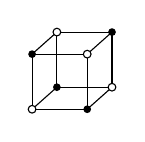
\begin{tikzpicture}[scale=.7]
\draw (0,0)--(1,0)--(1,1)--(0,1)--cycle;
\draw (.45,.4)--(1.45,.4)--(1.45,1.4)--(.45,1.4)--cycle;
\draw (0,0)--(.45,.4) (1,0)--(1.45,.4) (1,1)--(1.45,1.4) (0,1)--(.45,1.4);
\fill (0,1) circle (.07) (1,0) circle (.07) (.45,.4) circle (.07) (1.45,1.4) circle (.07);
\draw[fill=white] (0,0) circle (.07) (1,1) circle (.07) (.45,1.4) circle (.07) (1.45,.4) circle (.07);
\end{tikzpicture}}&\substack{\text{ou encore des}\\
\text{deux couleurs (échangées}\ldots\text{)}\\
\text{des faces de}\\\text{l'octaèdre }\Delta}\end{array}
&
\substack{\text{correspond au car.}\\\text{non trivial de}\\\{1,\underline a_\Delta\}}
&
\substack{\text{correspond}\\\text{au caractère}\\\text{non trivial}\\
\text{de }\mathrm{Aut}_{\mathrm{oct}}^+(\Delta)}\\
\begin{array}{cl}\figure{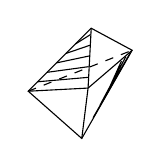
\begin{tikzpicture}[scale=.8]
\draw (0,0)--(1,1)--(1.65,.65)--(.85,-.75)--cycle;
\draw (1,1)--(.95,.05)--(.85,-.75) (0,0)--(.95,.05)--(1.65,.65);
\draw[dashed] (0,0)--(1.65,.65);
\draw (.15,.15)--(.95,.22) (.3,.3)--(.96,.39) (.45,.45)--(.97,.56) (.6,.6)--(.98,.73) (.75,.75)--(.99,.9);
\draw (1.03,-.42)--(1.62,.61) (1.14,-.22)--(1.55,.55) (1.25,-.03)--(1.48,.48);
\end{tikzpicture}}&\substack{\text{correspond.}\\\text{du car. }\deleted{\unsure{\mathrm{sg}\times\det}}\\
\text{de }\mathrm{Aut}_{\mathrm{oct}}^+(\Delta)\times\{1,\underline a_\Delta\}}\end{array}
&&\\
\substack{\uline{\text{NB}}\ \text{On a }F(\Delta)\simeq C_\Delta\times I_\Delta\\
\text{où }I_\Delta=F(\Delta)/\underline a_\Delta\ \text{est l'ens.}\\
\text{des quatre directions de faces}}
&&
\end{array}}
\right.
\]



qui satisfont à un iso. canonique
\[
(41)\qquad
\deleted{\unsure{\mathrm{Or}_\Delta}}\ \mathrm{Or}(\Delta)
\wedge\underbrace{\underline\omega_\Delta}\wedge C_\Delta
\simeq1_{\mathbb{F}_2}.
\]

On a un isom.
\[
(42)\quad
\left\{\begin{array}{l}
C_\Delta=\displaystyle\bigwedge_{i\in J}\Delta_i
\quad\text{quotient de }
\overset{\text{torseur sous }\mathbb{F}_2^J}{\overbrace{\displaystyle\prod_{i\in J}\Delta_i=F(\Delta)}}\\
\qquad\text{pour }\ 
\diagram{\begin{tikzcd}
\mathbb{F}_2^J\arrow[r,"\text{(somme)}"]\arrow[d,equal]&\mathbb{F}_2\\
\underset{M_0}{\underbrace{V_J(\mathbb{F}_2)}}\times\mathbb{F}_2&
\end{tikzcd}}\\
\text{i.e.}\quad C_\Delta=
\underset{\substack{(P_M/(M_0\times\unsure{Z|\mathbb{F}_2})\deleted{\unsure{/M_0}}\text{ dans le cas qui nous occupe})\\
\text{correspond au car. }\mathrm{sg}(g)\cdot\det(g)\text{ dans le cas où}\\
\Delta\text{ est défini par un }M)}}
{\underbrace{F(\Delta)/M_0}}
\end{array}\right.
\]
\margin{donc dans ce cas on a $C_\Delta\simeq\underline\mu\wedge\underline\omega$}

\deleted{(40)}
\[
(43)\qquad
\underline\omega_\Delta=\underline\omega_{I_\Delta}=\underline\omega_J
\quad\text{l'ens à deux éléments associé à }J
\]
(correspond au caractère $\mathrm{sg}(g)$ dans le cas d'un $M$)

\[
(44)\qquad
\deleted{\unsure{\underline\omega}}\ \mathrm{Or}(\Delta)
\simeq
\underset{\underline\omega_J}{\underbrace{\underline\omega_\Delta}}\wedge C_\Delta
\]
\margin{(correspond au caractère $\det(g)$ dans le cas d'un $M$) donc
$\boxed{\mathrm{Or}(\Delta)\simeq\underline\mu^{\det}=(\det M)^*}$.}

L'octaèdre \uline{orienté} \inserted{$\Delta^+$} associé à $M$ est défini par le torseur $P_M/\mathbb{F}_2^{\underline\omega}$ sous $M_0=V_J(\mathbb{F}_2)$, i.e. par

\scanpage{37}
\mspage{18}
% archive foliation: 36

$F(\Delta)/\{1,\underline a_\Delta\}$ (cf (36)), qui est donc l'ens des quatre bifaces de $\Delta$. Donc c'est l'octaèdre orienté canoniquement associé à l'octaèdre $\Delta$, savoir
\[
(45)\quad
\left\{\begin{array}{l}
\Delta^+=\deleted{\unsure{\Delta_\Delta\wedge\mathbb{F}_2}}\mathrm{Or}(\Delta)\wedge_{\{1,\underline a_\Delta\}}\Delta\\
\Delta=\mathrm{Or}(\Delta)\wedge_{\{1,\underline a_\Delta\}}\Delta^+
\end{array}\right.
\]
de sorte qu'on a \inserted{bien}, comme il se doit
\[
(\unsure{45|46})\quad
\left\{\begin{array}{l}
\mathrm{Or}(\Delta^+)\simeq\{\pm1\}=1_{\mathbb{F}_2}\\
\underline\omega_{\Delta^+}\simeq\underline\omega_\Delta\simeq\underline\omega_J=\underline\omega
\quad[\text{car }\underline a_\Delta\text{ opère trivialement sur }\underline\omega_\Delta]\\
C_{\Delta^+}\simeq C_\Delta\wedge\underline\mu\simeq\underline\omega\qquad\ldots
\end{array}\right.
\]

$\big[\big[$ Il importe maintenant de bien comprendre la structure d'extension
\[
(47)\qquad
\diagram{\begin{tikzcd}
1\arrow[r]&\underset{\{\pm1\}}{\underset{\simeq}{Z}}\arrow[r]&
GL(M)\arrow[r]&
\underset{\substack{\mathrm{Aut}_{\mathrm{oct}}(\Delta_M)'\\
\simeq\mathrm{Aut}_{\mathrm{oct}}^+(\Delta_M)\times\{1,\underline a_{\Delta_M}\}}}
{\underset{\simeq}{GL(M)'}}\arrow[r,dash]&1
\end{tikzcd}}
\]
et en particulier
\[
(48)\qquad
\diagram{\begin{tikzcd}
1\arrow[r]&\underset{\{\pm1\}}{\underset{=}{Z_0}}\arrow[r]&
GL(2,\mathbb{Z}/4\mathbb{Z})\arrow[r]&
\underset{\substack{\mathrm{Aut}_{\mathrm{oct}}(\Delta_{(\mathbb{Z}/4\mathbb{Z})^2})\\
\text{``octaèdre standart''}}}
{\underset{\simeq}{GL(2,\mathbb{Z}/4\mathbb{Z})'}}\arrow[r,dash]&1
\end{tikzcd}}
\]
puisque c'est par là qu'on comprend quelle est la donnée supplémentaire qu'il faut pour déduire, d'un octaèdre non orienté $\Delta$, le $(\mathbb{Z}/4\mathbb{Z})$-module libre de rang $2$ $M$ dont $\Delta$ proviendrait — question qui revient à celle de ``remonter'' un torseur sous le groupe $GL(2,\mathbb{Z}/4\mathbb{Z})'$ en un torseur sous le groupe $GL(2,\mathbb{Z}/4\mathbb{Z})$ lui-même.

\scanpage{38}
% archive foliation: 37

Je me reporte au diagramme (23)
\[
\diagram{\begin{tikzcd}[column sep=large]
&&1\arrow[d]&&\\
&&\mathbb{F}_2^{\underline\omega}\arrow[dl]\arrow[dr,equal]&&1\arrow[dl]\\
&GL_\Lambda(M)\arrow[dl]\arrow[dr]&&\mathbb{F}_2^{\underline\omega}\simeq V(S_Q)\arrow[dl]&\\
\unsure{\mathcal{G}_I|\mathfrak S_I}\arrow[dr,"\inserted{\mathrm{sg}}"']&
\text{cart}&\mathfrak D_Q\arrow[dl,"\chi_C"]&\\
&\{\pm1\}&&
\end{tikzcd}}
\]
qui exprime $GL_\Lambda(M)$ comme produit fibré, la donnée de $M$ équivalant à celle du triple $(I,Q,k)$, où $I$ est un ens. à quatre éléments, $Q$ un carré \inserted{combinatoire}, et $k$ un isom
\[
k:\underset{\text{codiagonales}}{\underbrace{C_Q}}
\ \simeq\ \underline\omega_I.
\]

En termes de $Q$, on a
\[
C_\Delta\simeq F(\Delta)/M_0\simeq
P_{M,\mathbb{F}_2^{\underline\omega}}/\mathbb{F}_2
=S_Q/\mathbb{F}_2\simeq D_Q
\]
ens des diagonales de $Q$ — donc la donnée de l'octaèdre $\Delta$ (au lieu de $M\longleftrightarrow(I,Q,k)$) équivaut à celle de $I$, et des deux ens. à deux éléments $C$ $(\simeq\underline\omega_I)$ et $D$ correspondant aux diagonales et codiagonales du carré $Q$, \deleted{\unsure{dont}} la donnée équivaut à celle d'un torseur sous
$\deleted{\unsure{\mathfrak D_Q}}\mathfrak D_4/Z(\mathfrak D_4)\simeq\deleted{\unsure{\mathbb{F}_2}}\mathbb{F}_2\times\mathbb{F}_2$,
qu'il faut donc relever en un torseur sous $\mathfrak D_4$. Ou encore, décrire la donnée d'un carré combinatoire, dont on a déjà les deux ensembles \inserted{$C$ et $D$} (des \uline{codiagonales} et \uline{diagonales}\ldots\quad$\big]\big]$

\scanpage{39}
% archive foliation: 38

\uline{Récapitulation partielle}

A un module $M$ libre de rang $2$ sur $\mathbb{Z}/4\mathbb{Z}$ on associe

\[
(49)\quad
\left\{
\diagram{\begin{array}{p{.88\linewidth}}
a) L'octaèdre (non orienté) \inserted{de sommets} $\Delta_M=M^*/\pm1$, l'ens des trois diagonales s'identifiant à $(M/2M)^*\simeq M_0^*=J$\\[1em]
b) L'ensemble à quatre éléments $I$, qu'on peut p.ex. déduire de $\Delta$ comme
\[
I_M\simeq
\underset{\substack{\text{faces de }\Delta\\\unsure{\text{ou sections de }\Delta\text{ sur }J}}}
{\underbrace{F(\Delta)}}/\text{antipodisme}
\]\\
c) Le carré $Q_M$ \inserted{d'ens de sommets} $\unsure{S_M}=P_M/M_0$, où $P_M$ est le $\mathrm{End}(M_0)$-torseur formé des sections de $M^*$ sur $M_0^*$ satisfaisant $\xi_i+\xi_j+\xi_k=0$, et où on identifie $\mathrm{End}(M_0):M_0\oplus\mathbb{F}_2^{\underline\omega}$, de sorte que $P_M/M_0$ est un $\mathbb{F}_2^{\underline\omega}$ torseur, donc est l'ens des sommets d'un carré \inserted{$Q=Q_M$} dont l'ens des codiagonales est $\underline\omega$.
\end{array}}
\right.
\]

\margin{On a un iso. can.
$J\simeq\mathcal P_{2,2}(I_M)$,
$I_M$ torseur sous $\underset{(\simeq\mathbb{F}_2^J/\mathbb{F}_2)}{\underbrace{V_J(\mathbb{F}_2)\simeq M_0}}$
$I_M\simeq P_M/\mathbb{F}_2^{\underline\omega}$.}

\margin{\uline{NB} $F(\Delta)\simeq I\times
\underset{\text{``couleurs'' des faces}}{\underset{\downarrow}{C_\Delta}}$}

\margin{où $\underline\omega\simeq\underline\omega_I\simeq\underline\omega_J$}

Les données a) et b) ne dépendent que de la \deleted{fibré} droite projective $X_M=\mathbb{P}(M)$ sur $\mathbb{Z}/4\mathbb{Z}$ ($\Delta$ est l'ens des p$^{\mathrm{ts}}$ de celle-ci, $J$ celui des p$^{\mathrm{ts}}$ de $(X_M)_0$, droite projective sur $\mathbb{F}_2$), mais non pas $Q_M$. On a les bijections canoniques
\[
(50)\quad
\left\{
\begin{array}{lll}
\underset{\text{codiag de }Q}{\underbrace{C_Q}}
\simeq
\underset{\deleted{\unsure{\text{orientations de }\Delta}}}{\underline\omega_\Delta}
\overset{\mathrm{déf}}{\simeq}\underline\omega_I\simeq\underline\omega_J
&\text{soit }\underline\omega\\
\underset{\text{diag de }Q}{D_Q}
\simeq
\underset{\text{``couleurs'' des faces}}{\underline C_\Delta}
\simeq\underline\omega\wedge\underline\mu
&\text{où }\underline\mu\text{ défini ci-dessous}\\
\underset{\text{or. de }Q}{\underline\omega_Q}
\simeq\underline{\mathrm{Or}}(\Delta)\simeq\det(M)^*
&\text{soit }\underline\mu
\end{array}
\right.
\]

